\section{Implementation}
The implementation section describes the process of constructing the directional audio system from the designs. This involves describing any deviations from the designs during implementation to achieve the desired goal of the subsystem.

\subsection{Circuit construction}
The circuits required for the directional audio system involve the construction of an analogue linear amplitude modulator using the AD633 as well the development of the power amplifier with the LM380 power amplifier.
\subsubsection{AD633 Linear amplitude modulator implementation}
The AD633 amplitude modulator was implemented as the designs intended on a breadboard. The circuit was powered by a ISO-Tech IPS 2303 2 channel DC power supply and supplied with the carrier wave by the Voltcraft FG1617 Function Generator.
The implemented circuit is shown in figure \ref{fig:mixerbb} where there circuit implemented circuit matches the design shown in figure \ref{fig:amCirc}.

\begin{figure}[ht!]
    \centering
    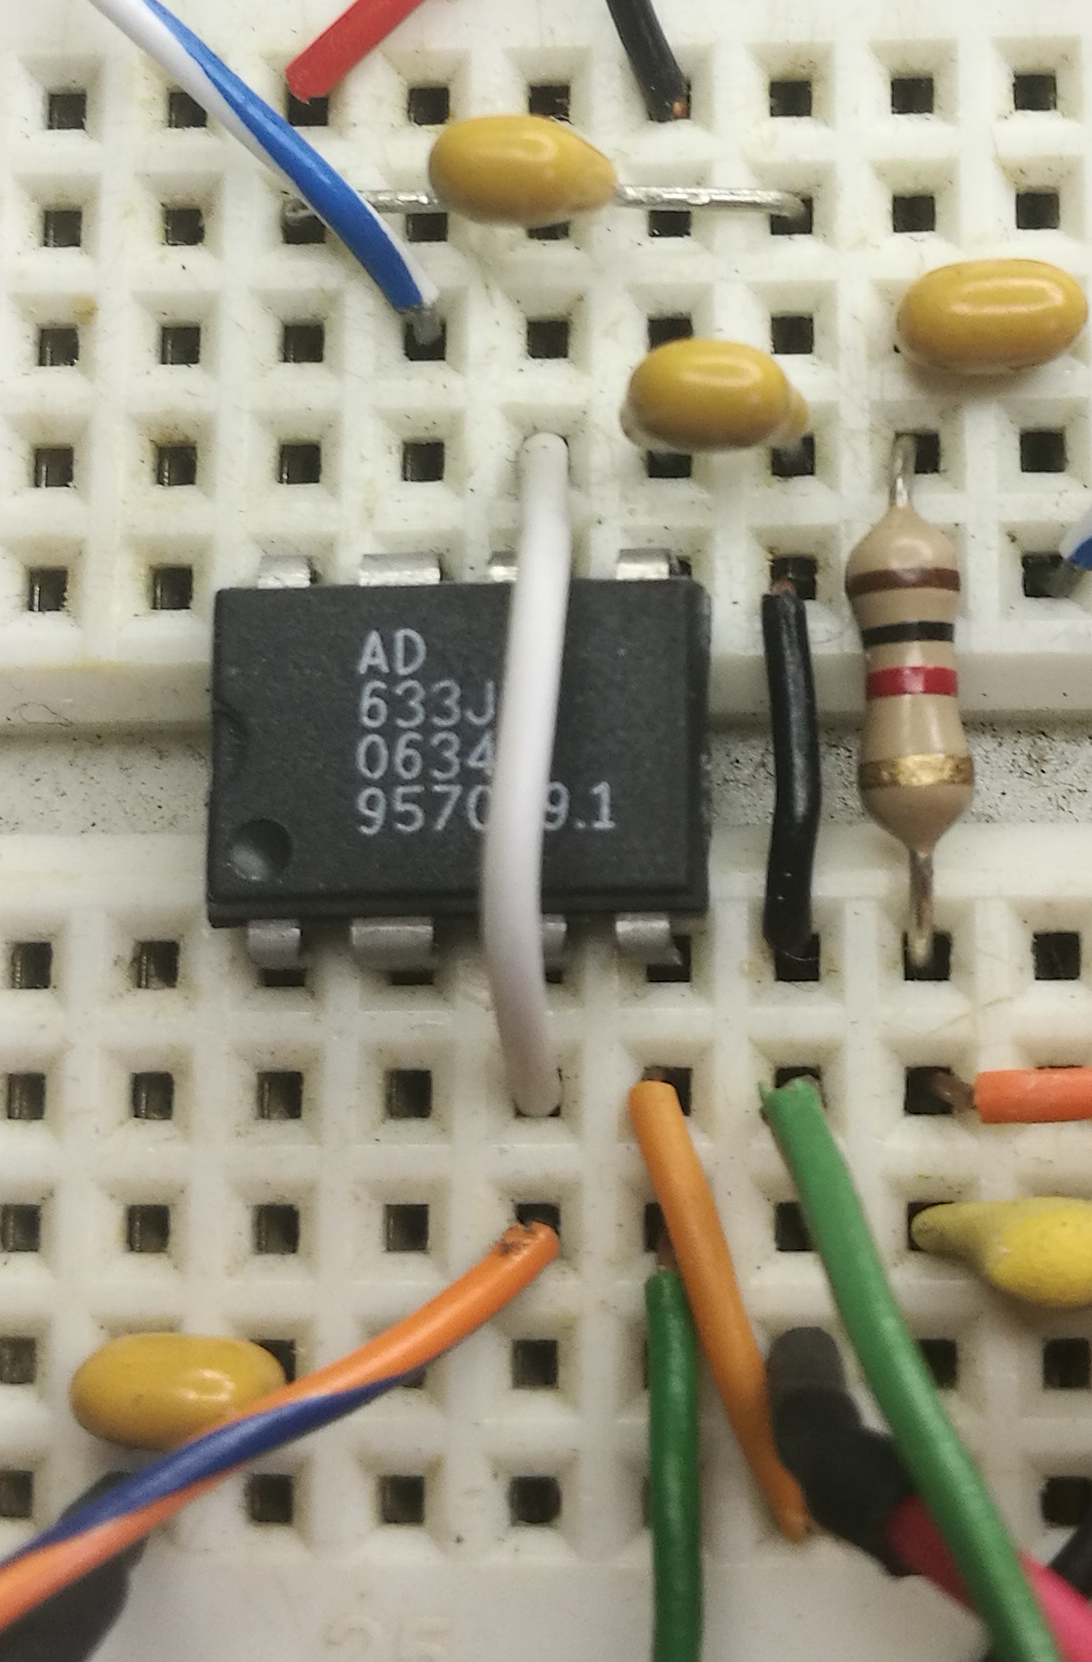
\includegraphics[width=0.3\textwidth]{Figures/Implementation/Mixer/mixerbboard.png}
    \caption{AM mixer implemented on breadboard}
    \label{fig:mixerbb}
\end{figure}

A test tone of 2.5 kHz is generated and input as the modulating waveform with a 40 kHz carrier input to the AD633 AM modulator and the outputs are shown in figure \ref{fig:mix2.5kinputVsOut} and \ref{fig:mix40kinputVsOut}.

\begin{figure}[ht!]
\centering

    \begin{minipage}{0.49\textwidth}
    \centering
    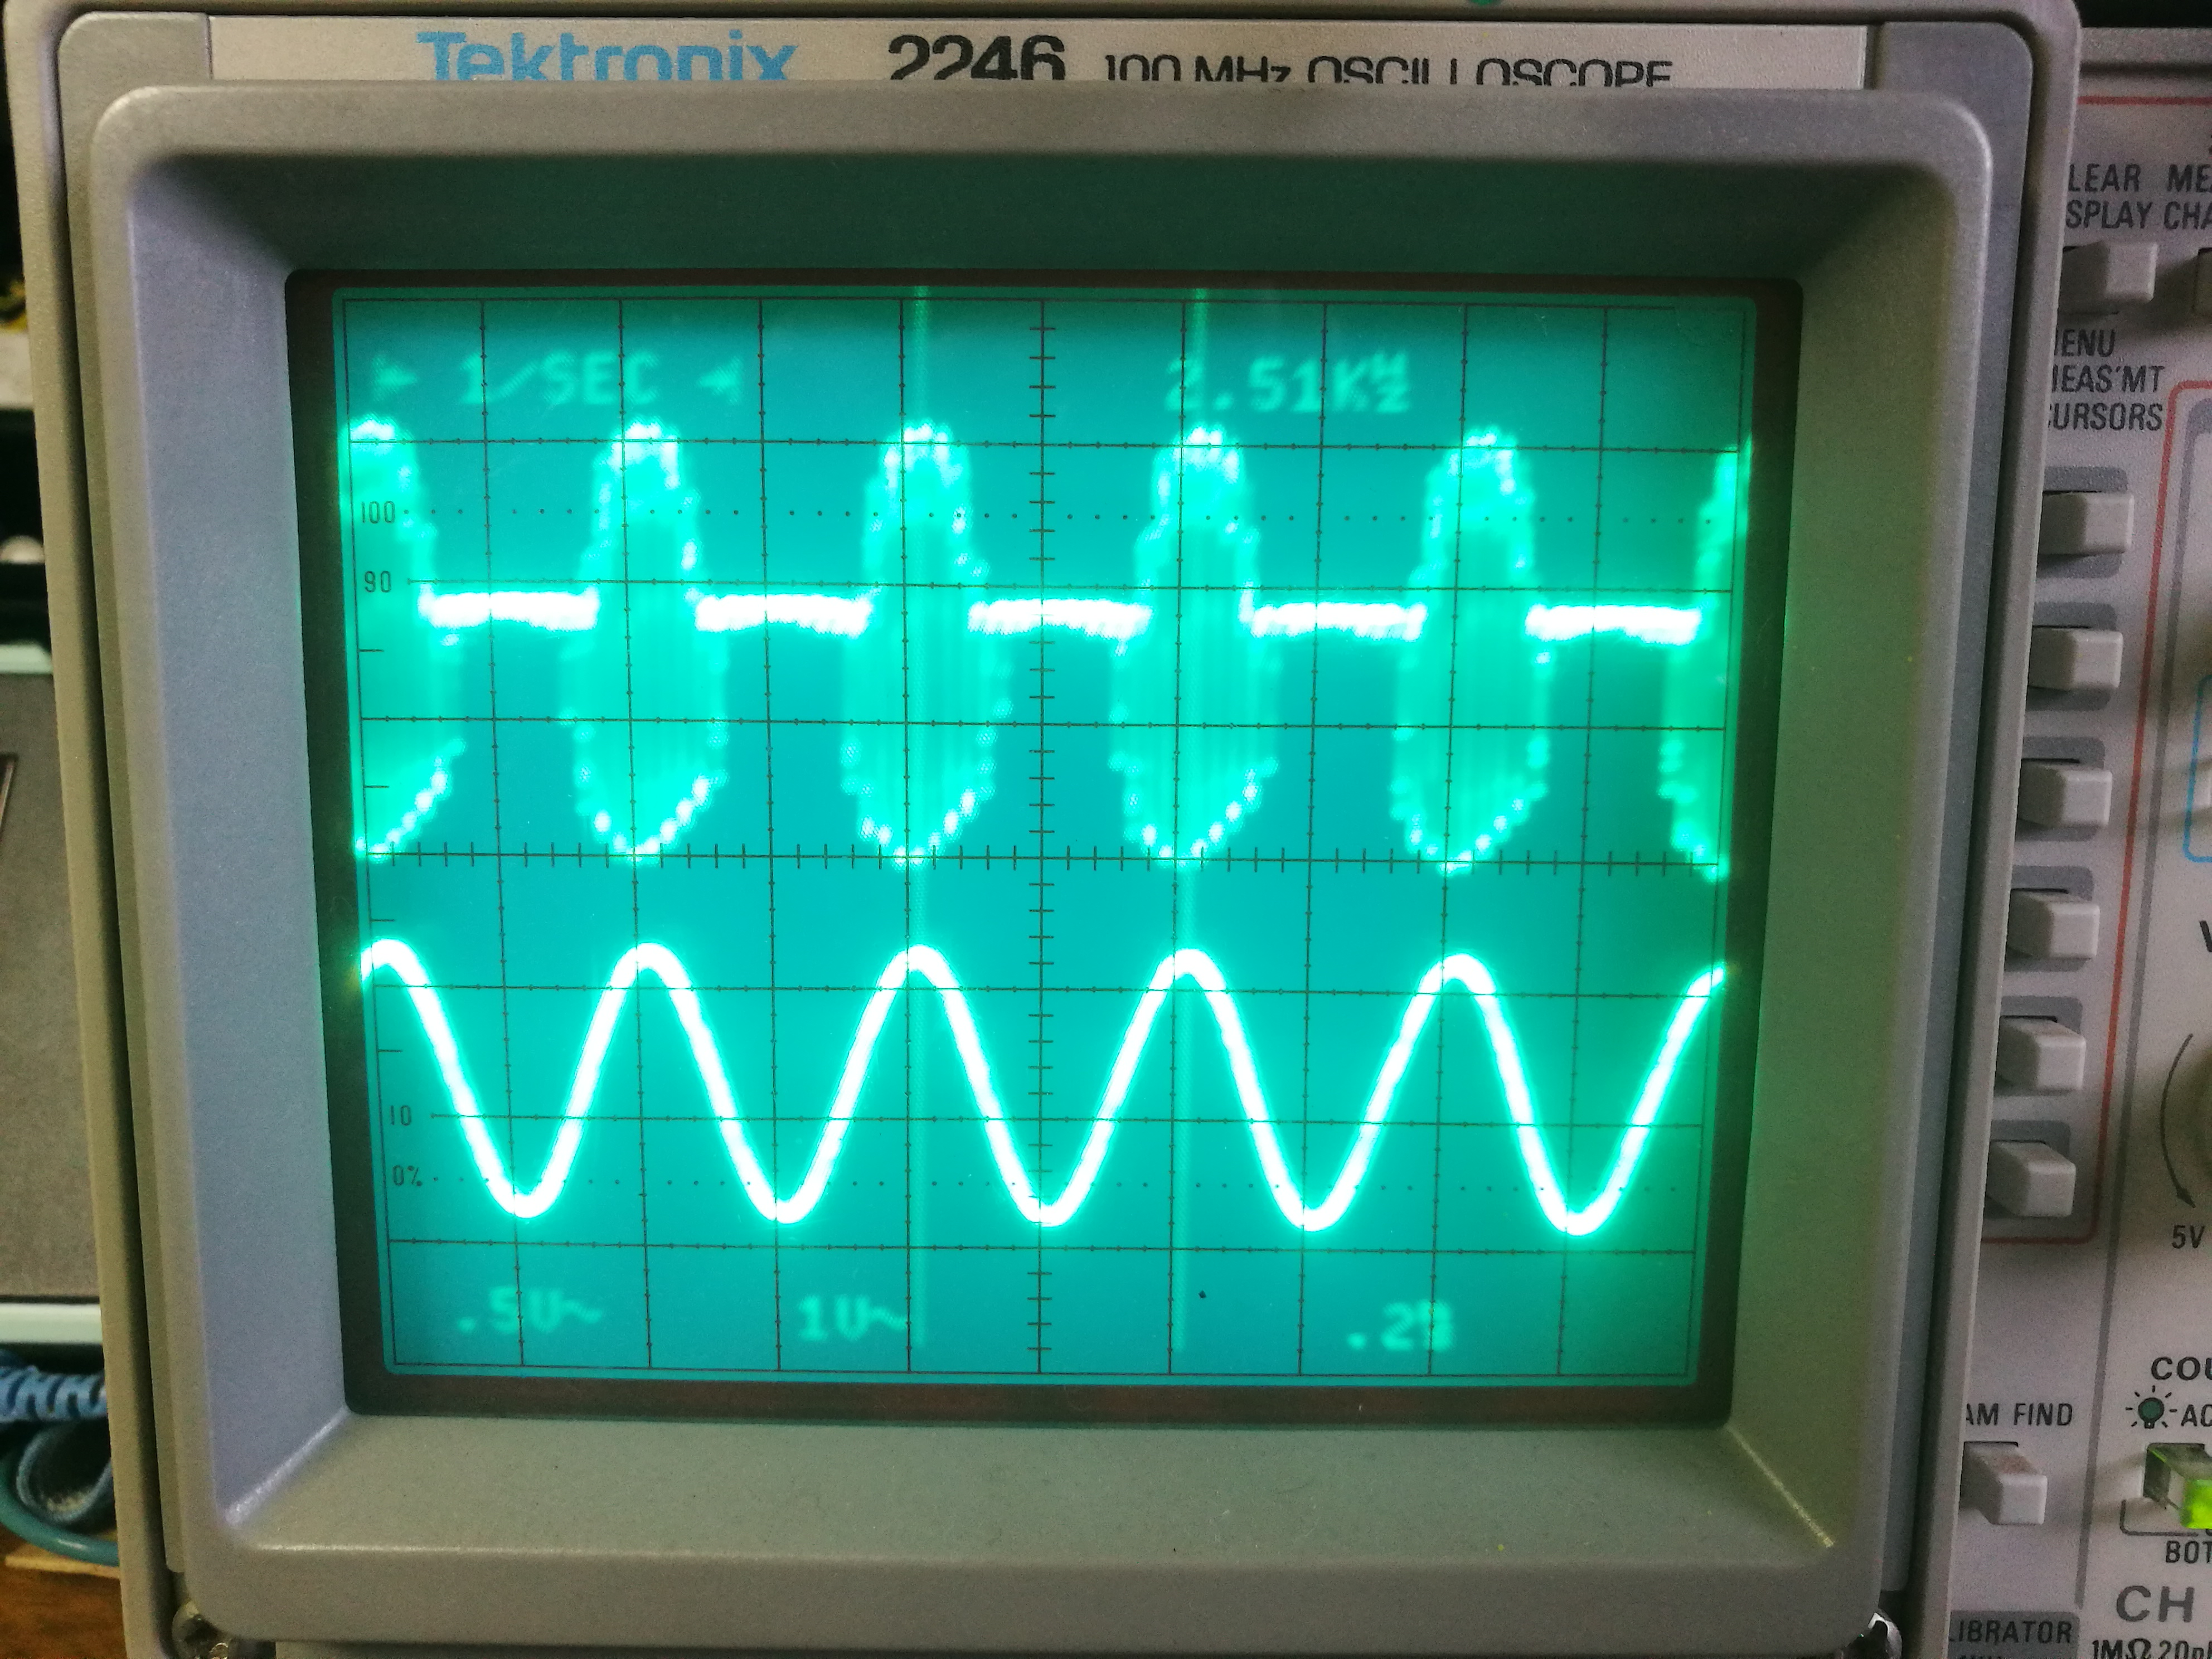
\includegraphics[width= \textwidth]{Figures/Implementation/Mixer/infreq.jpg}
    \caption{Input 2.5 kHz frequency compared to modulated output}
    \label{fig:mix2.5kinputVsOut}
    \end{minipage}\hfill
    \begin{minipage}{0.49\textwidth}
    \centering
    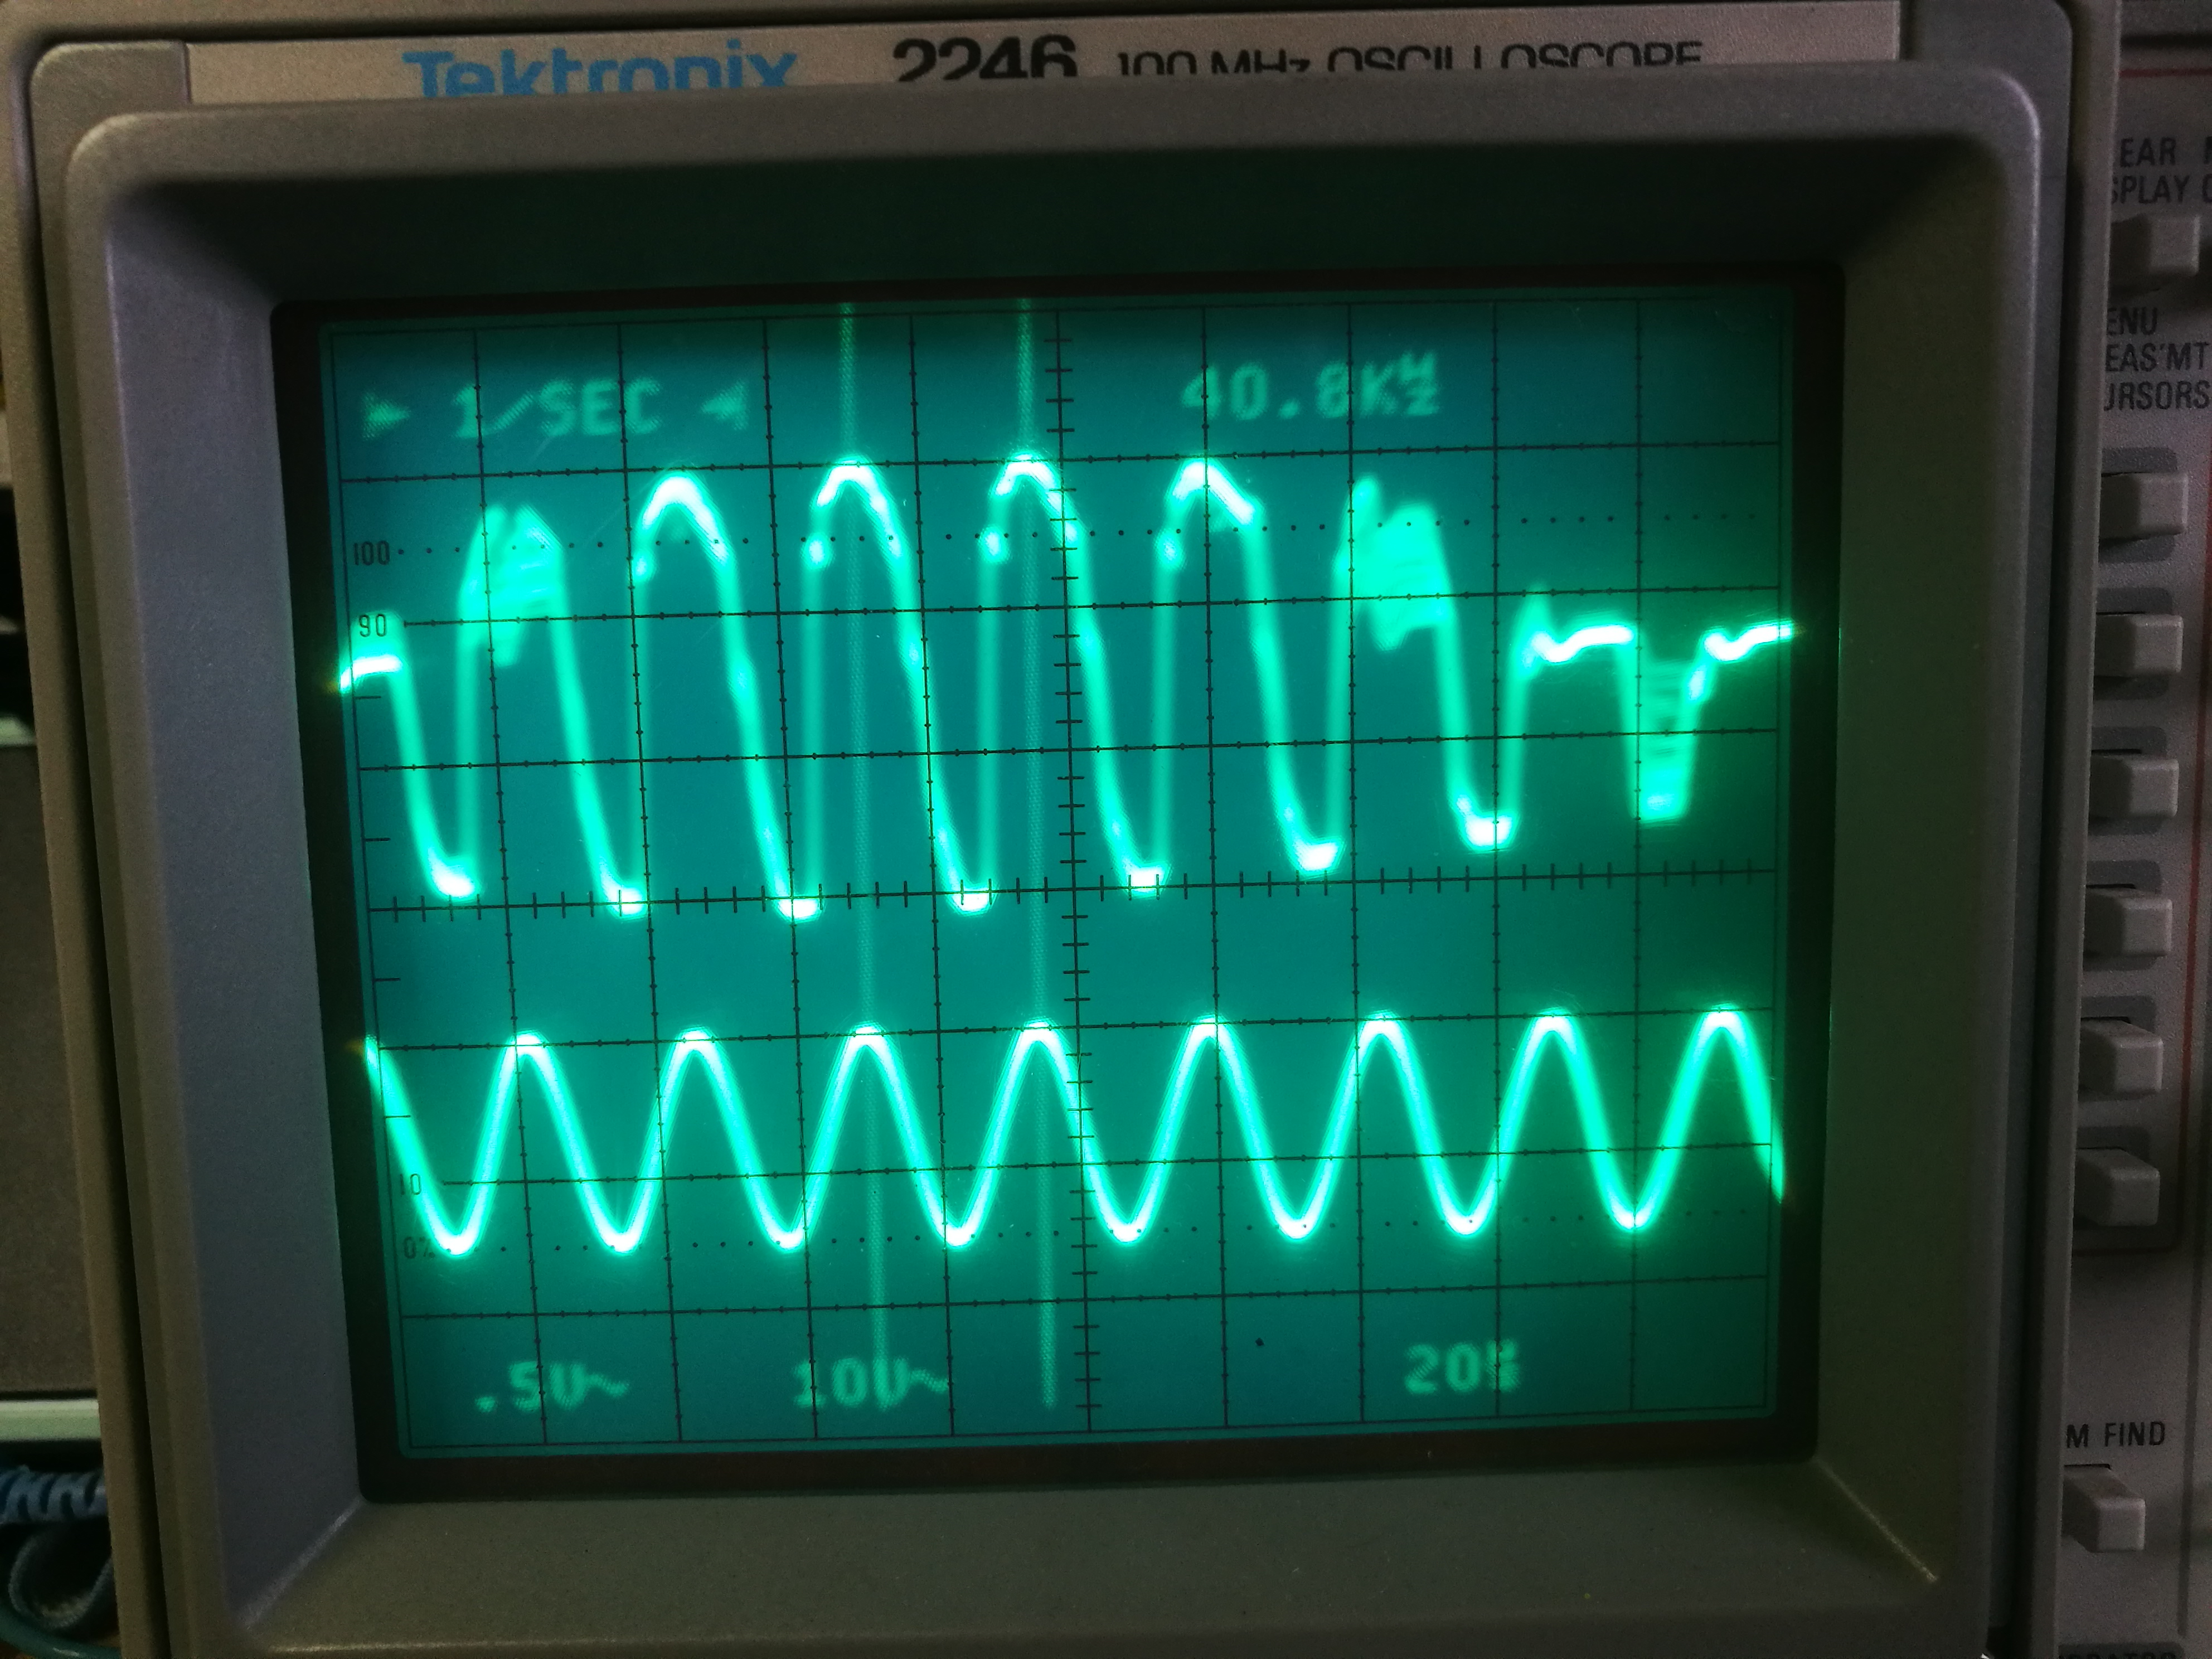
\includegraphics[width= \textwidth]{Figures/Implementation/Mixer/outfreq.jpg}
    \caption{Input 40 kHz frequency compared to modulated output}
    \label{fig:mix40kinputVsOut}
    \end{minipage}
    
\end{figure}

Figure \ref{fig:mixerinVsout} demonstrates the input modulating signal compared to the output AM signal. The output shows an approximate peak amplitude of 1.5V with a near zero amplitude for the negative half cycle. While this doesn't match up well with the expected output levels of the simulations; it is still an acceptable result for the subsystem. From these measurements the modulation index appears to lie around 50\% using equation \ref{eqn:modIndex} given a carrier amplitude of 1V.

\begin{figure}[ht!]
    \centering
    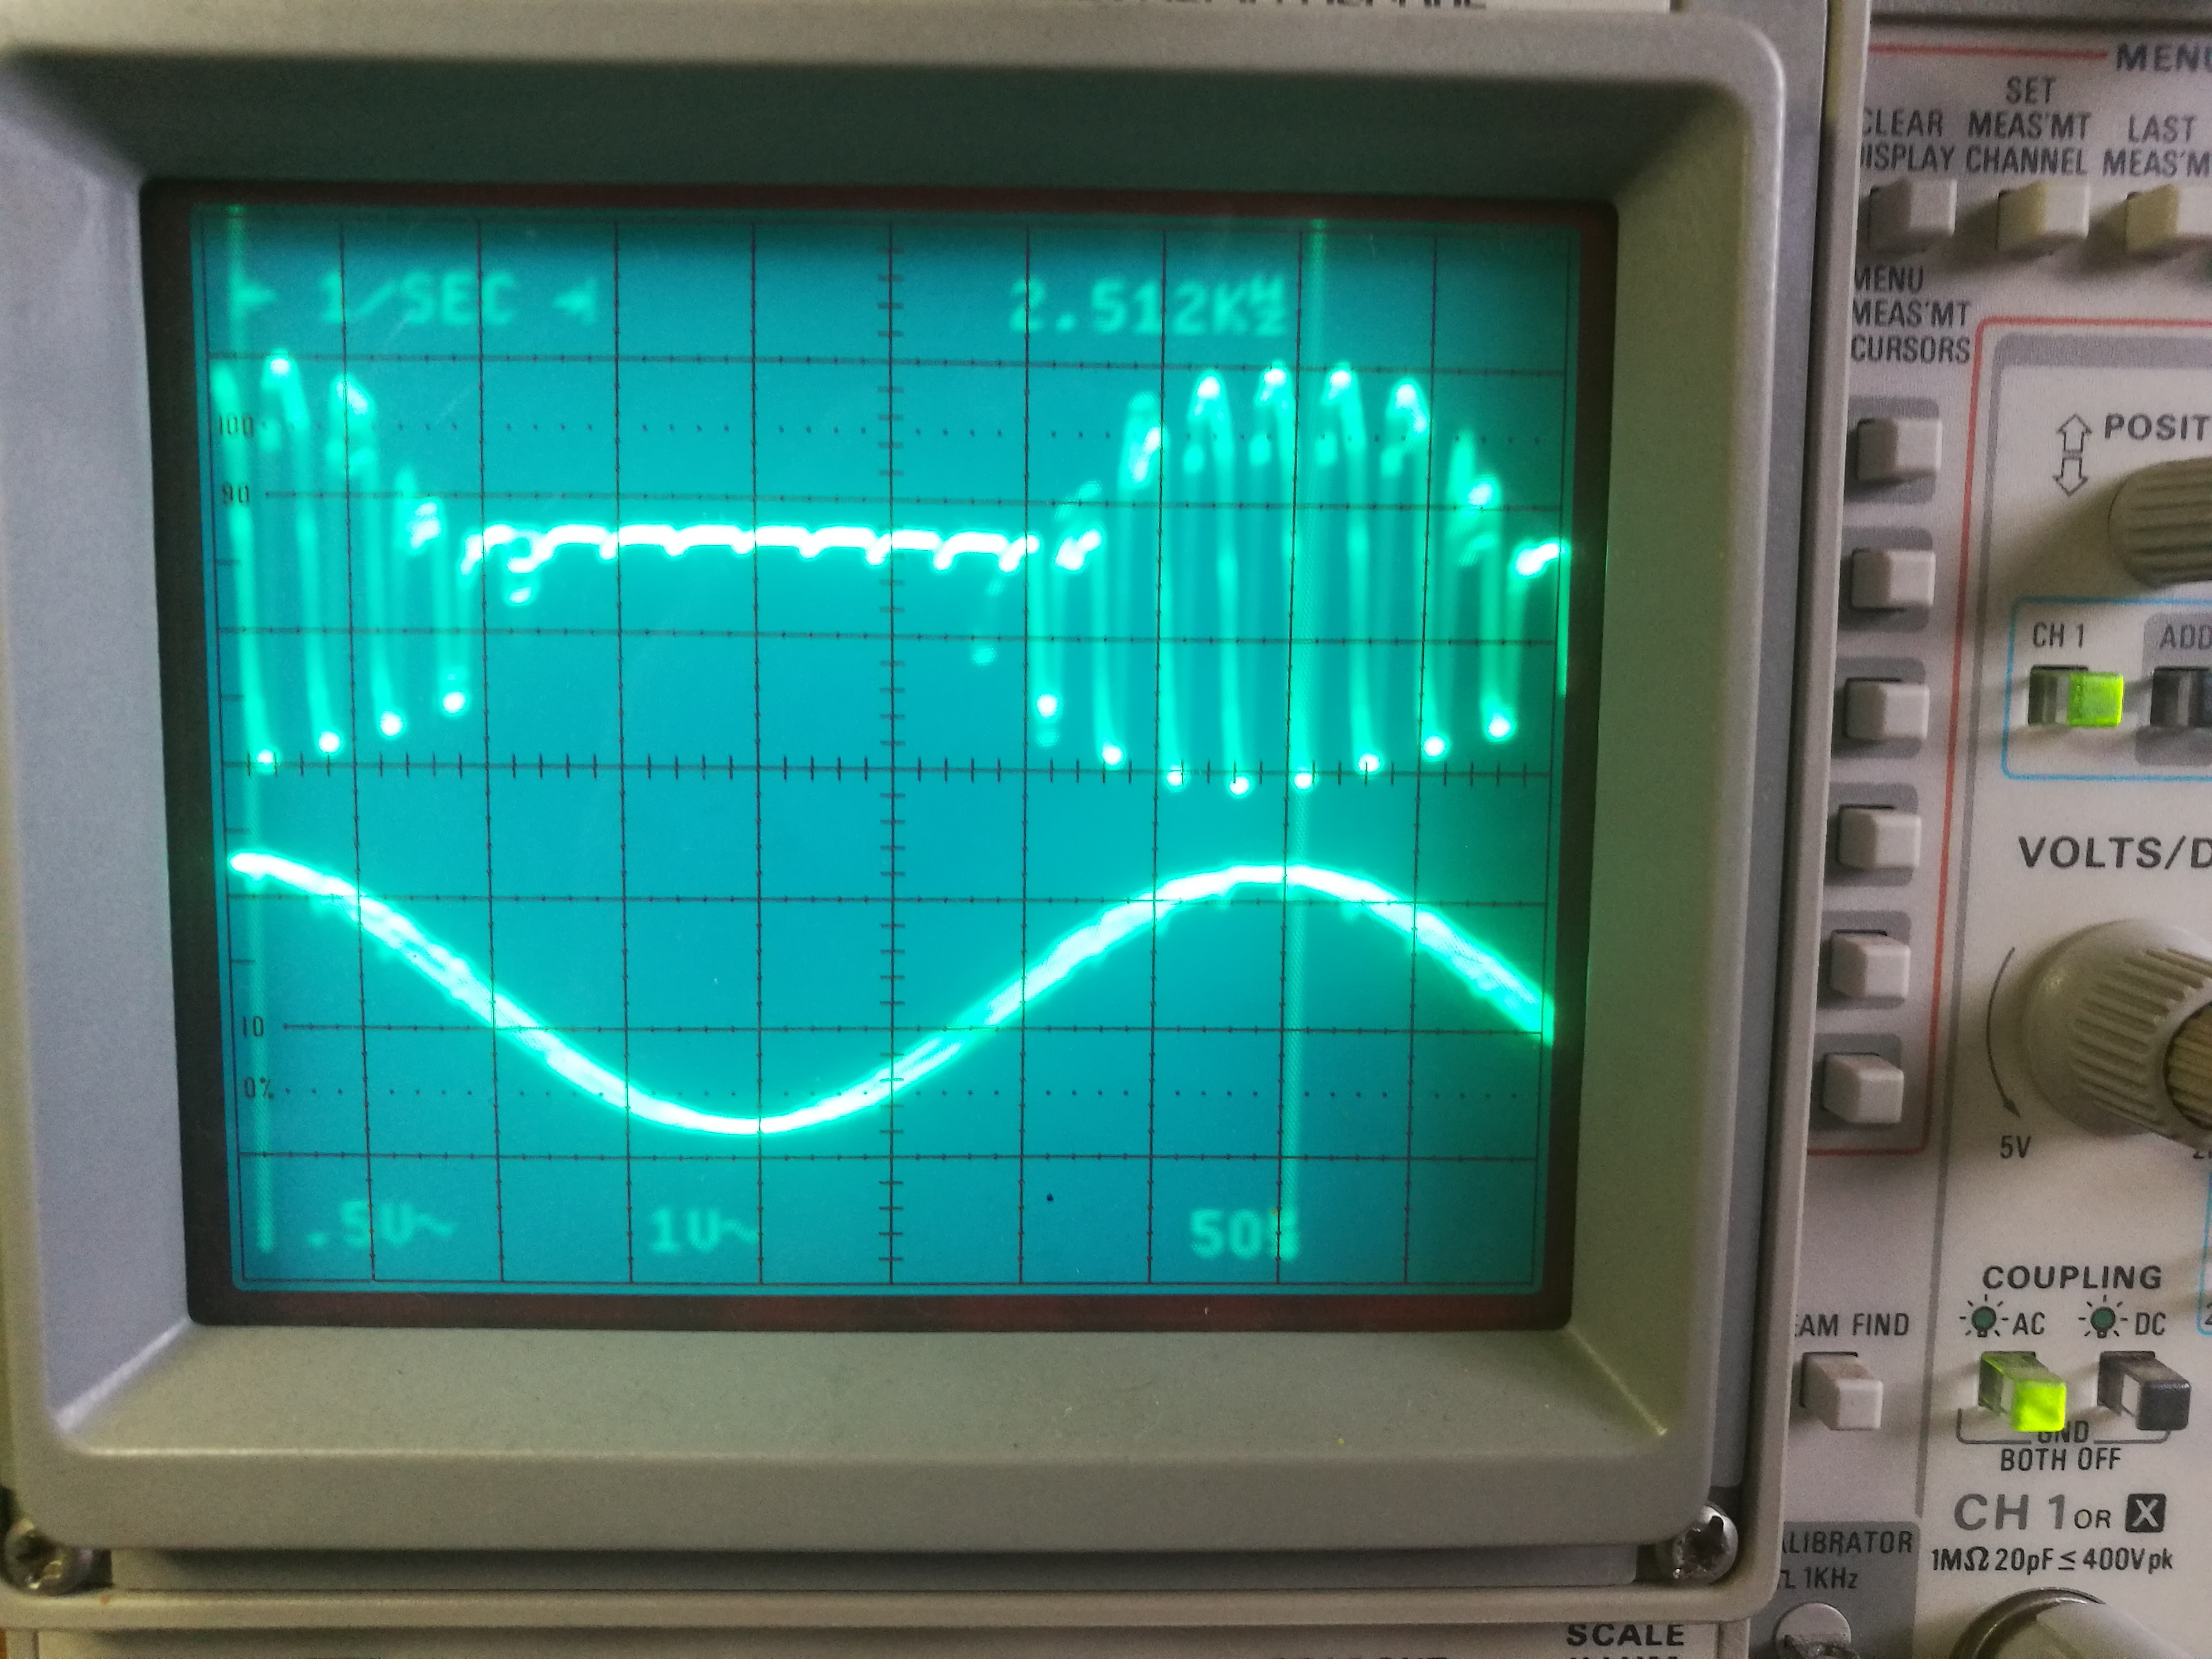
\includegraphics[width=0.8\textwidth]{Figures/Implementation/Mixer/mixoutVsin.jpg}
    \caption{AM mixer output versus input signal}
    \label{fig:mixerinVsout}
\end{figure}

\subsubsection{Amplifier Implementation}
The implementation of the amplifier involved many small tweaks from the original design due to a low frequency oscillations occurring on the output. As such the final implementation involves many more components that were used to reduce these low frequency oscillations during the troubleshooting process. Figure \ref{fig:ampbbCirc} demonstrates the end result from the troubleshooting where the oscillations were under control. Figure \ref{fig:ampCircPosttbl} illustrates the new circuit after troubleshooting the low frequency oscillations.

\begin{figure}[ht!]
    \centering
    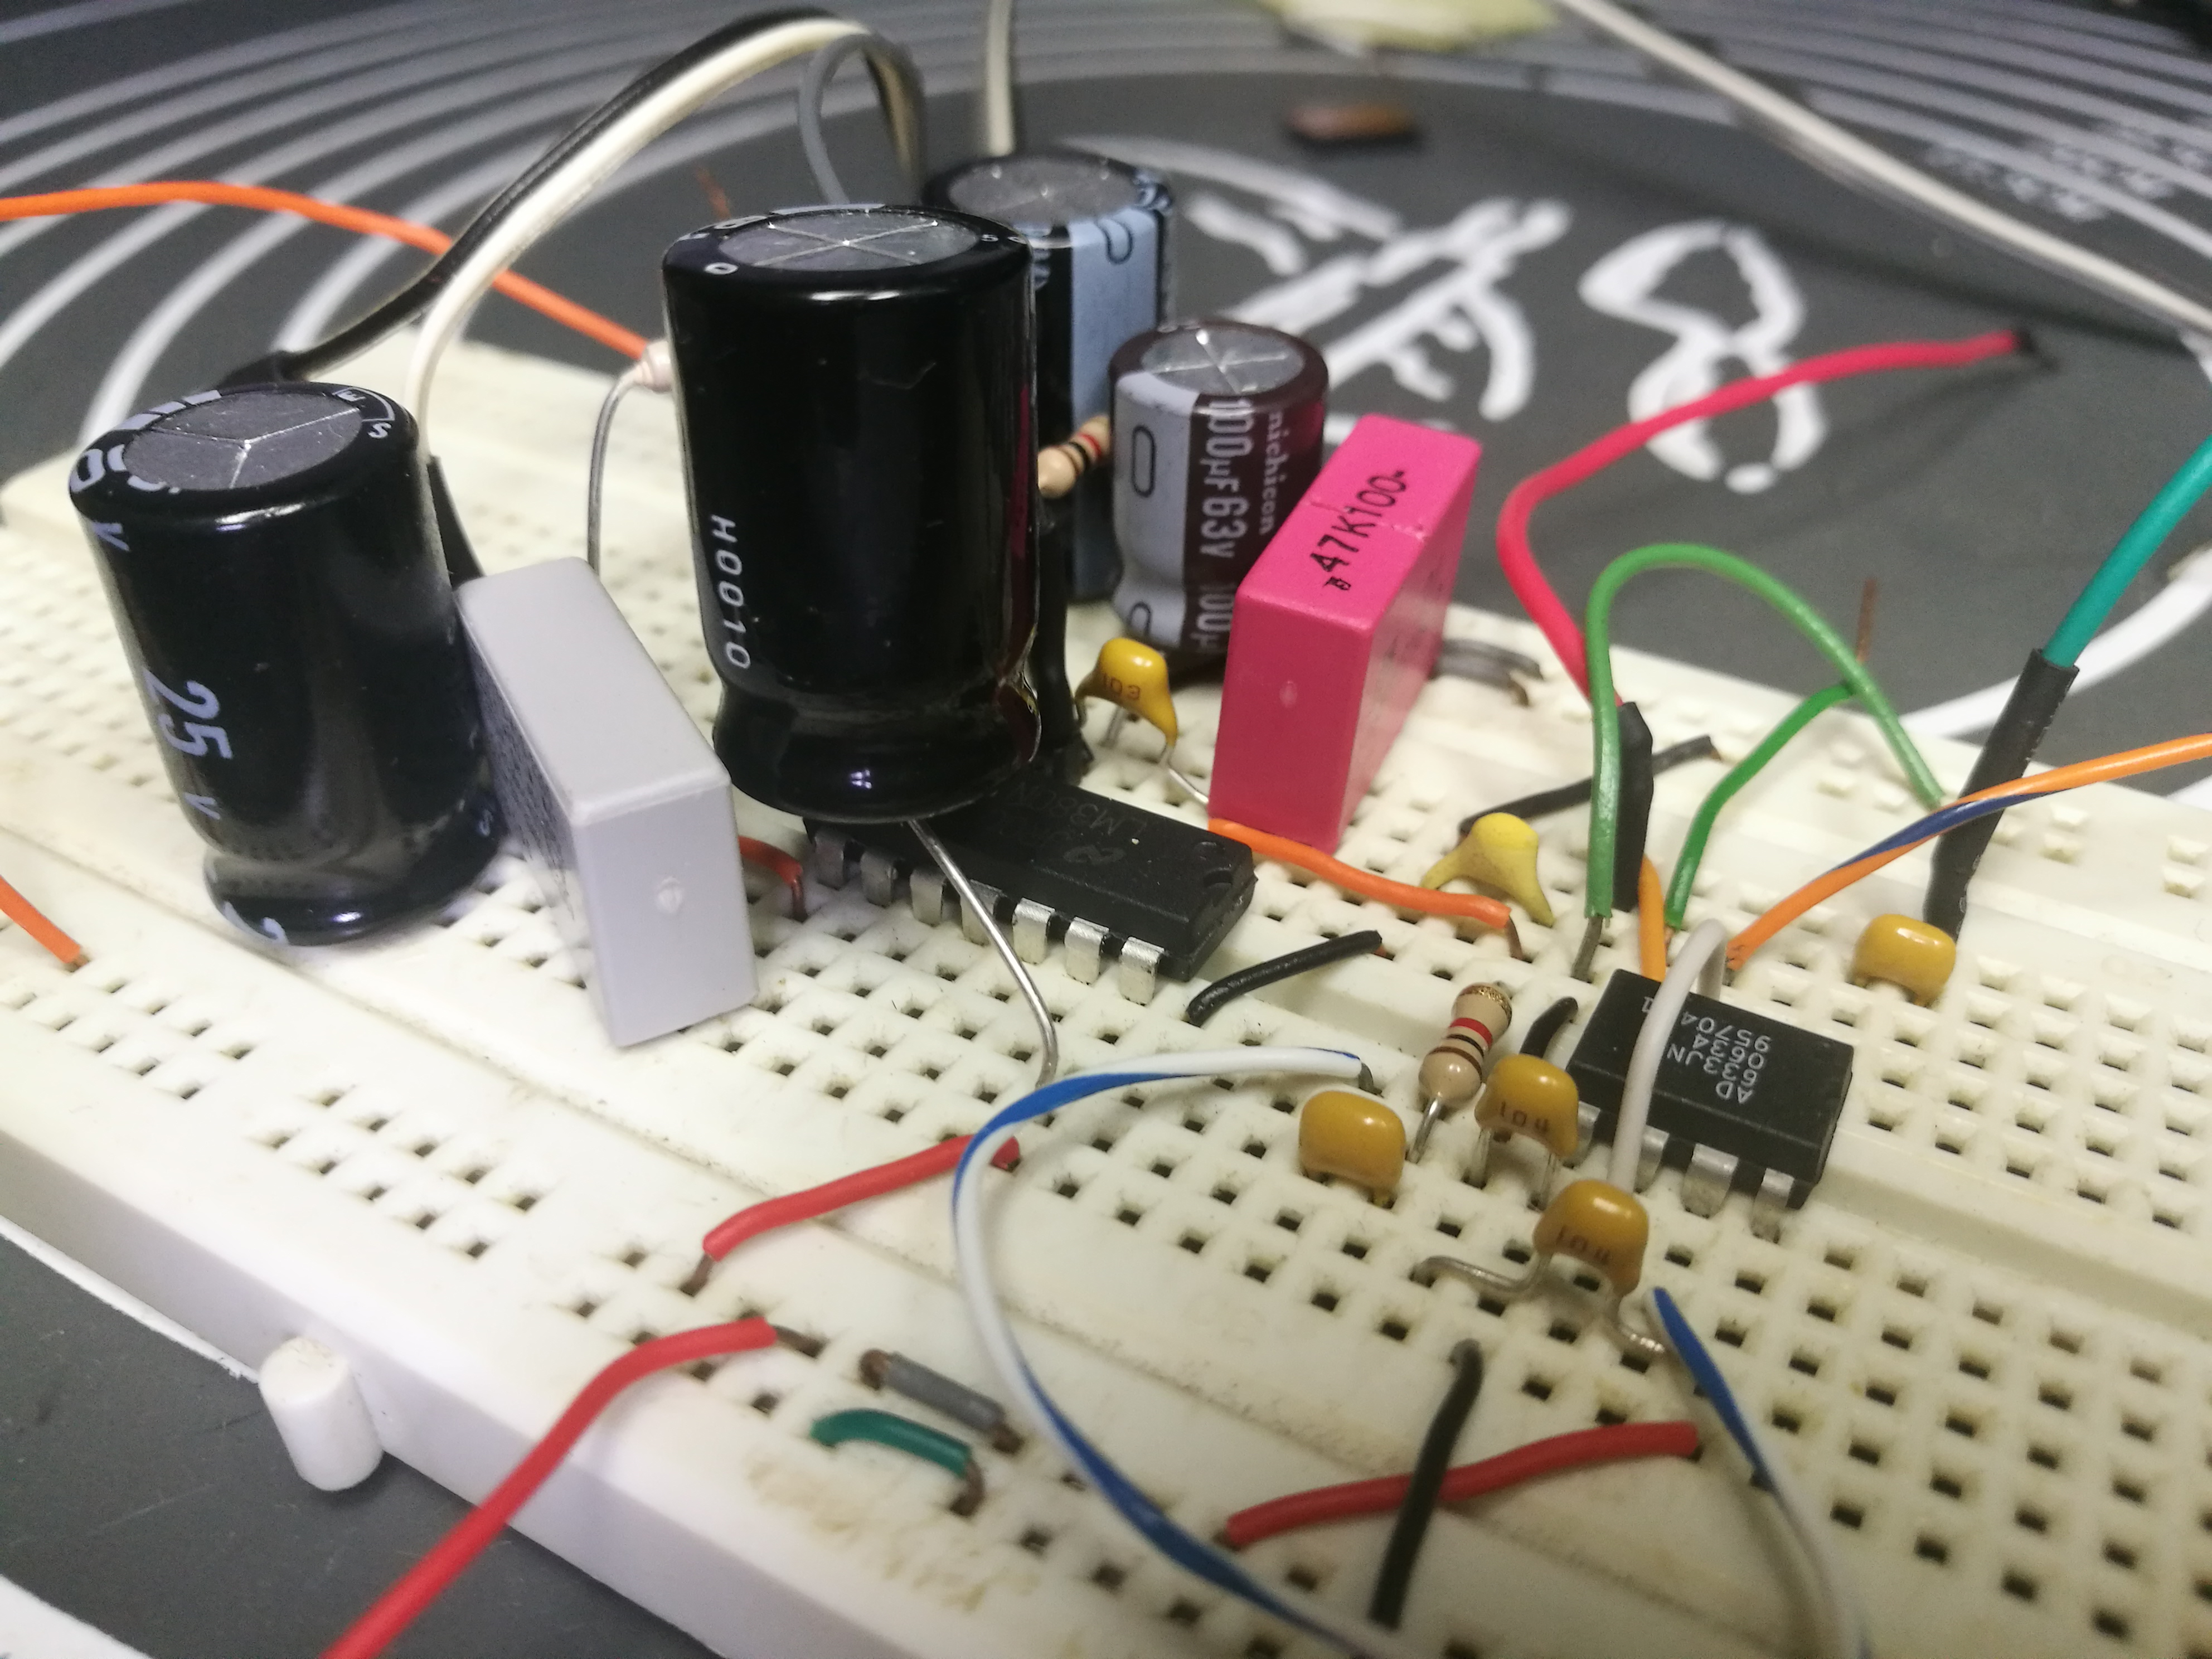
\includegraphics[width=0.8\textwidth]{Figures/Implementation/Amplifier/ampbbcirc.jpg}
    \caption{LM380 Power amplifier breadboard circuit after troubleshooting}
    \label{fig:ampbbCirc}
\end{figure}

\begin{figure}[ht!]
    \centering
    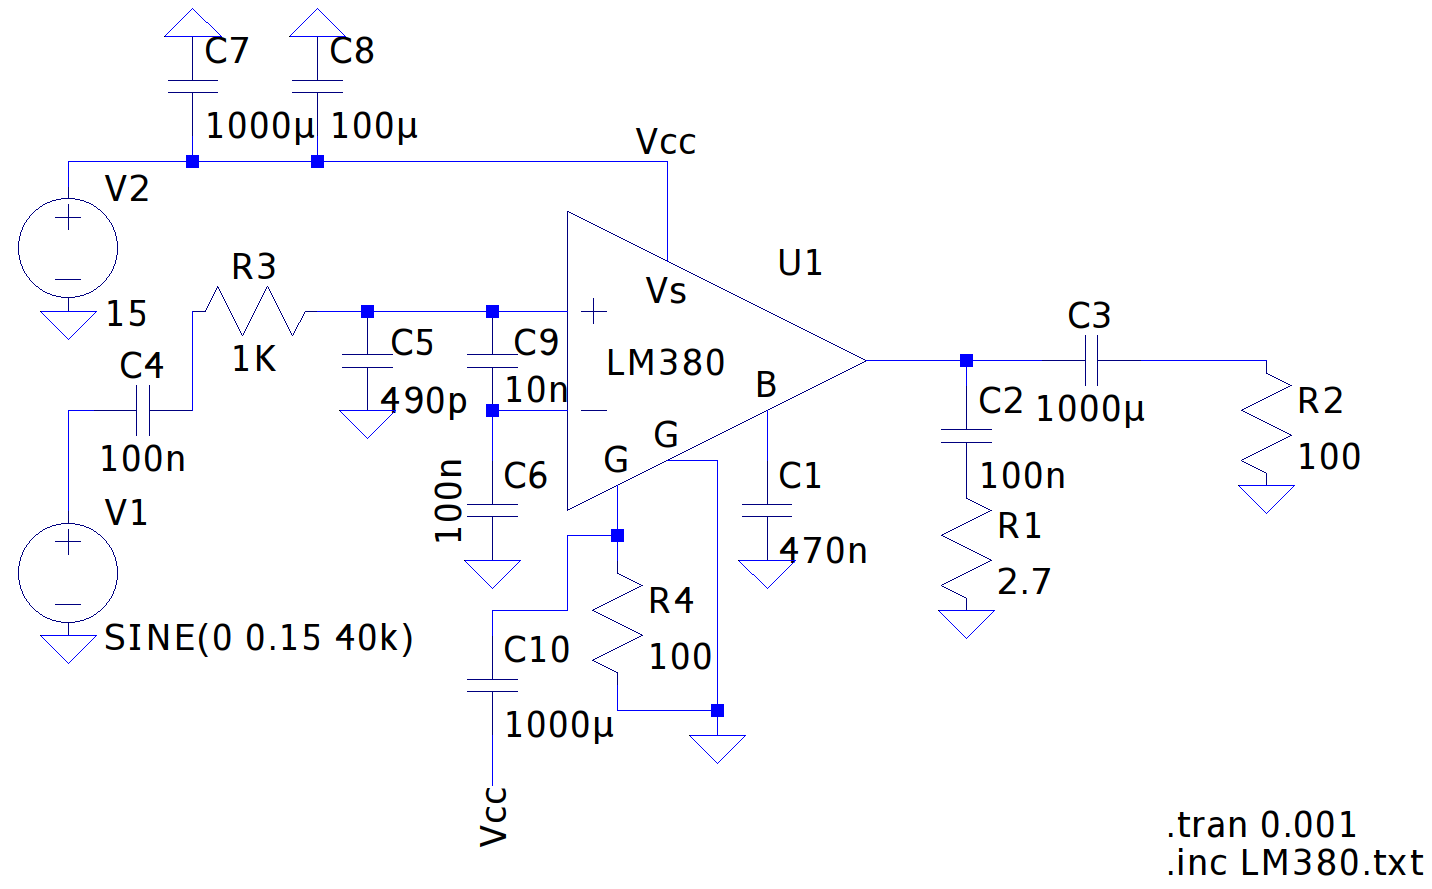
\includegraphics[width=0.8\textwidth]{Figures/Implementation/Amplifier/Lm380Mod.png}
    \caption{LM380 Power amplifier circuit schematic after troubleshooting}
    \label{fig:ampCircPosttbl}
\end{figure}

Upon application of a low frequency test tone of 500 Hz to a ordinary speaker, the amplifier produced an audible output with no low frequency oscillations. The output shown in figure \ref{fig:ampOscOut} demonstrates the resultant output of the amplifier. The output only shows the positive half cycle of the wave due to the electrolytic capacitor present on the output, blocking the negative half cycle. Unfortunately no alternative capacitors were readily available to correct this since the restrictions imposed by Covid-19 blocked access to components.
\begin{figure}[ht!]
    \centering
    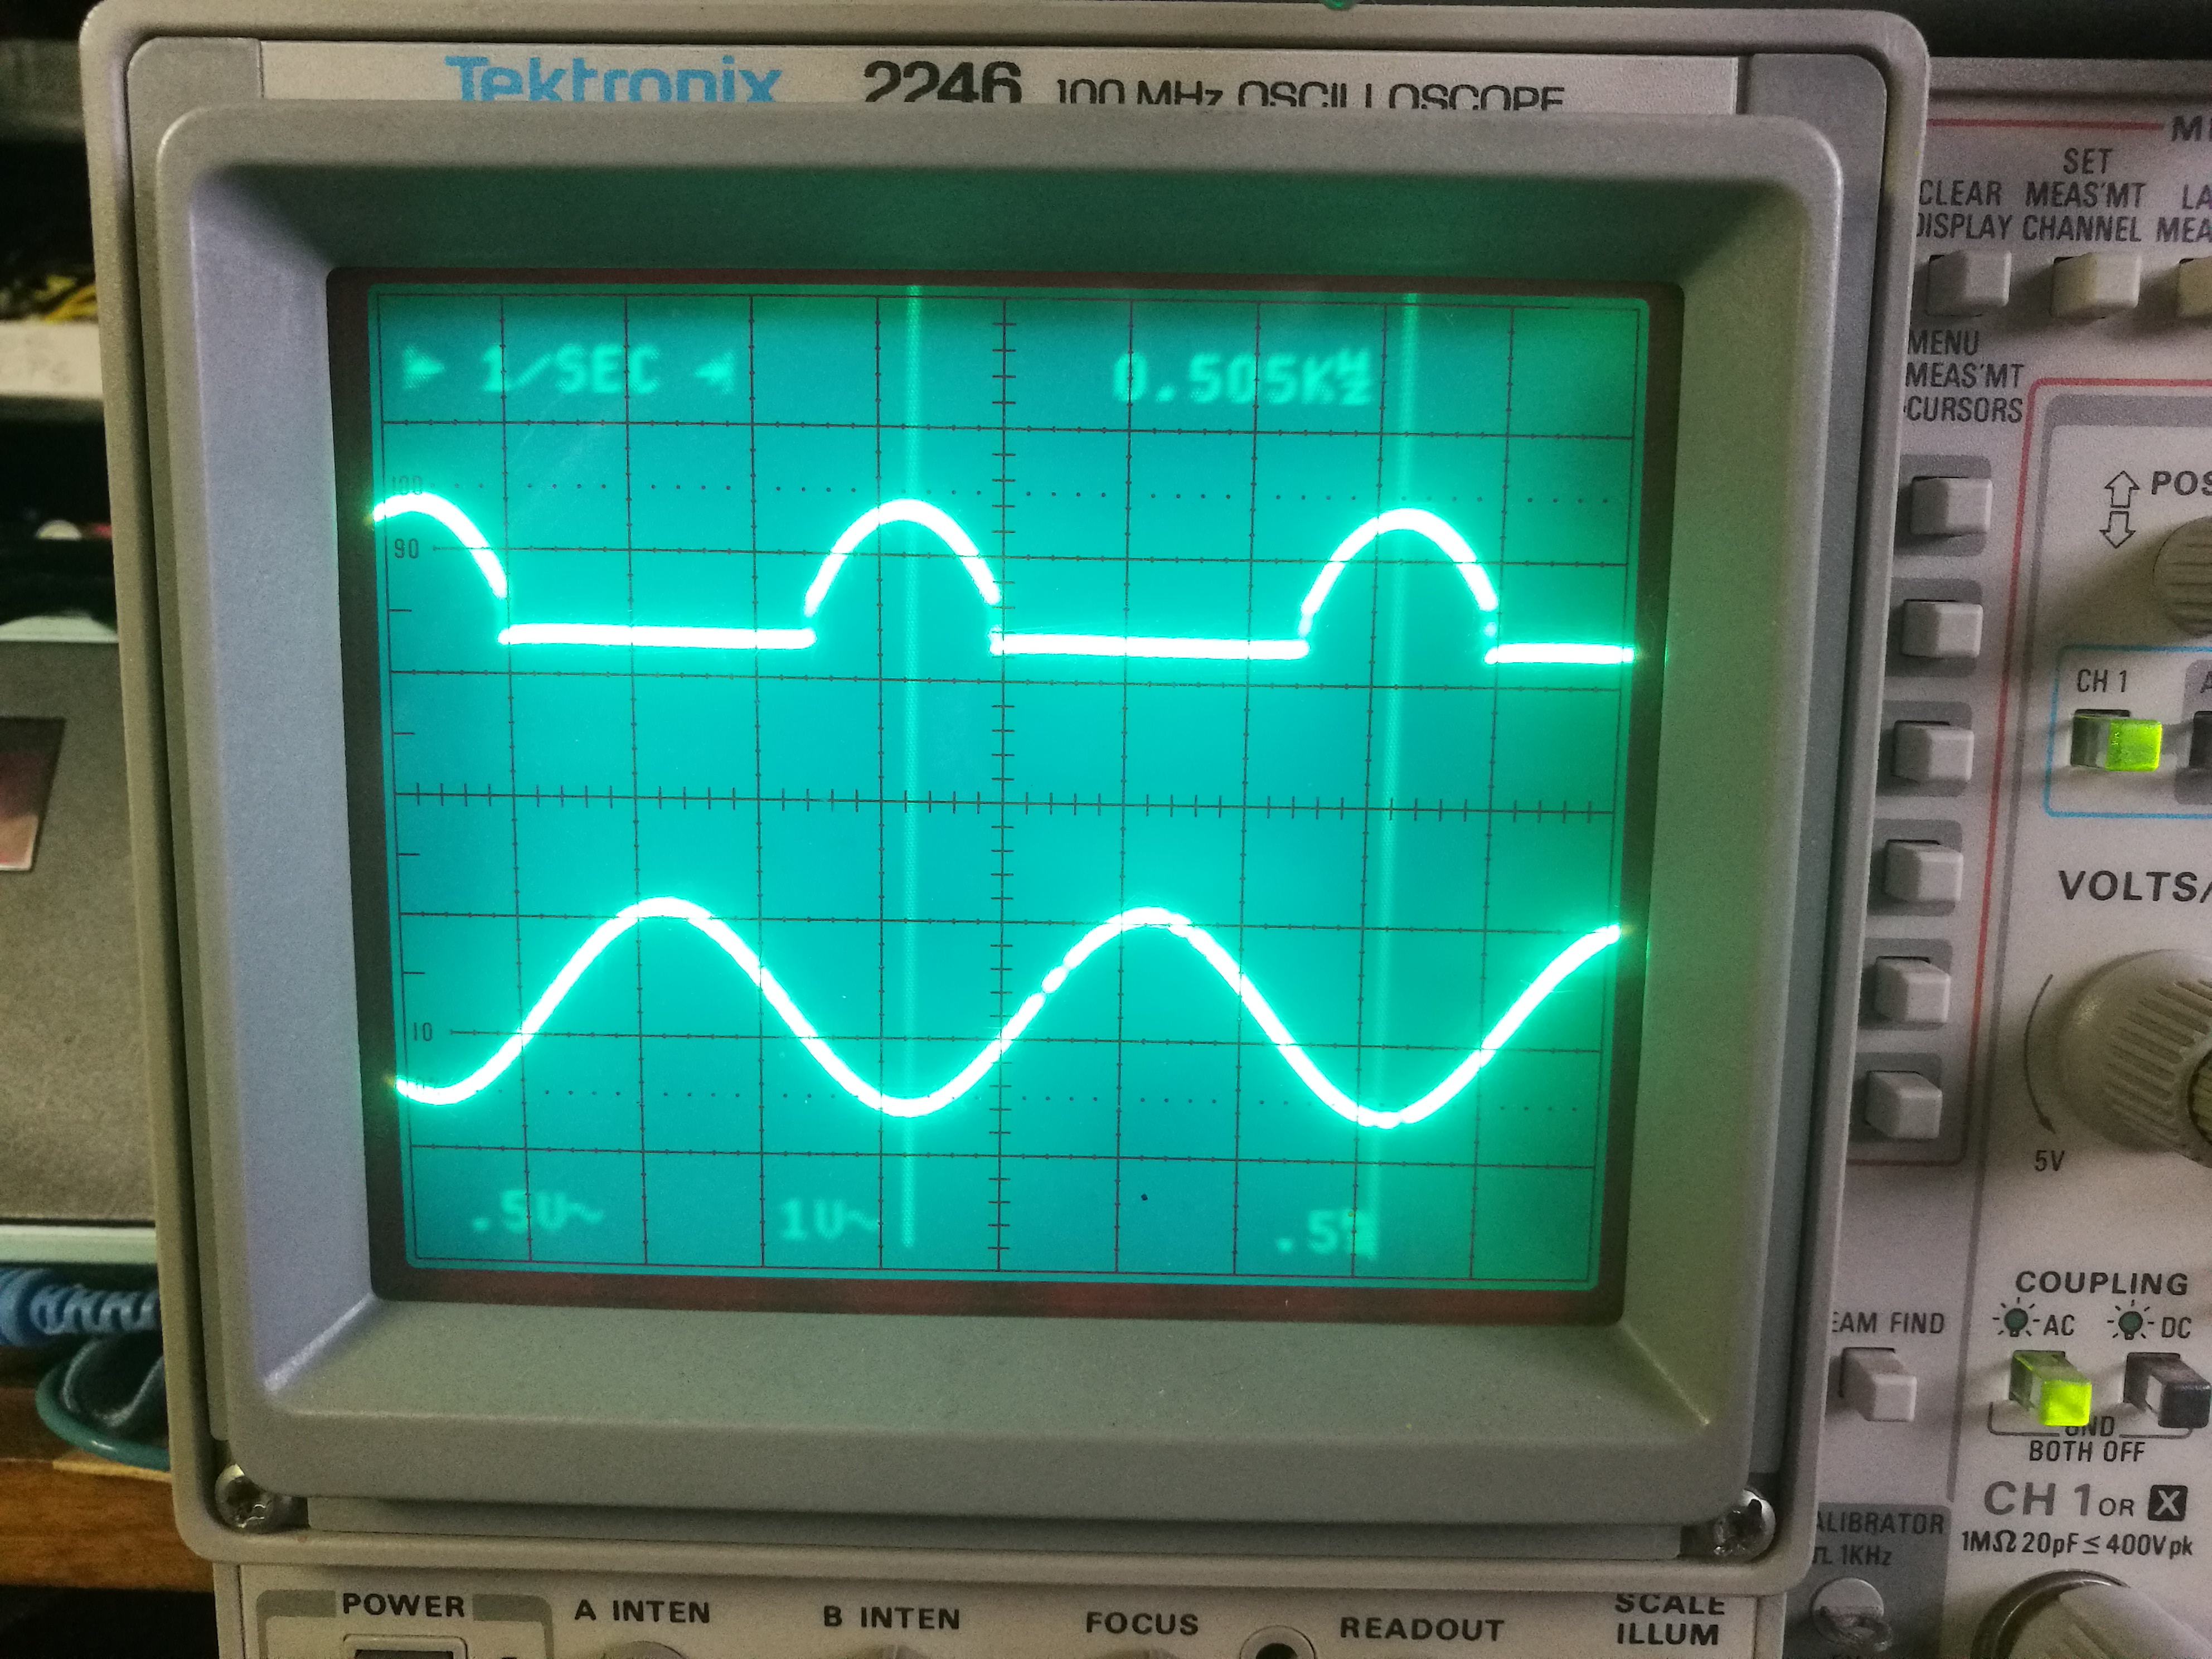
\includegraphics[width=0.8\textwidth]{Figures/Implementation/Amplifier/ampOutbb.jpg}
    \caption{LM380 Power amplifier 500 Hz output to test speaker}
    \label{fig:ampOscOut}
\end{figure}
Since the capacitor's main purpose is to smooth out the peeks for the 8 $\Omega$ speaker during this test, it can be bypassed when connecting the ultrasonic array.


\newpage
\subsection{Transducer array construction}
The construction of the transducer array began once the previously designed PCBs arrived from JLC PCB. 21 Kibitone 400ST ultrasonic transducers were placed into the spaces provided by the PCB paying careful attention transducer orientation and soldered in place. Figures \ref{fig:pcbfrontunpop} and \ref{fig:pcbbackunpop} show the unpopulated PCB and figures \ref{fig:pcbfront} and \ref{fig:pcbback} show the PCB populated with the ultrasonic transducers. Additionally; M4 bolts with foam spacers, metal washers and nuts can be seen in the back view which are used for mounting in the tripod during testing.

\begin{figure}[ht!]
\centering

    \begin{minipage}{0.49\textwidth}
    \centering
    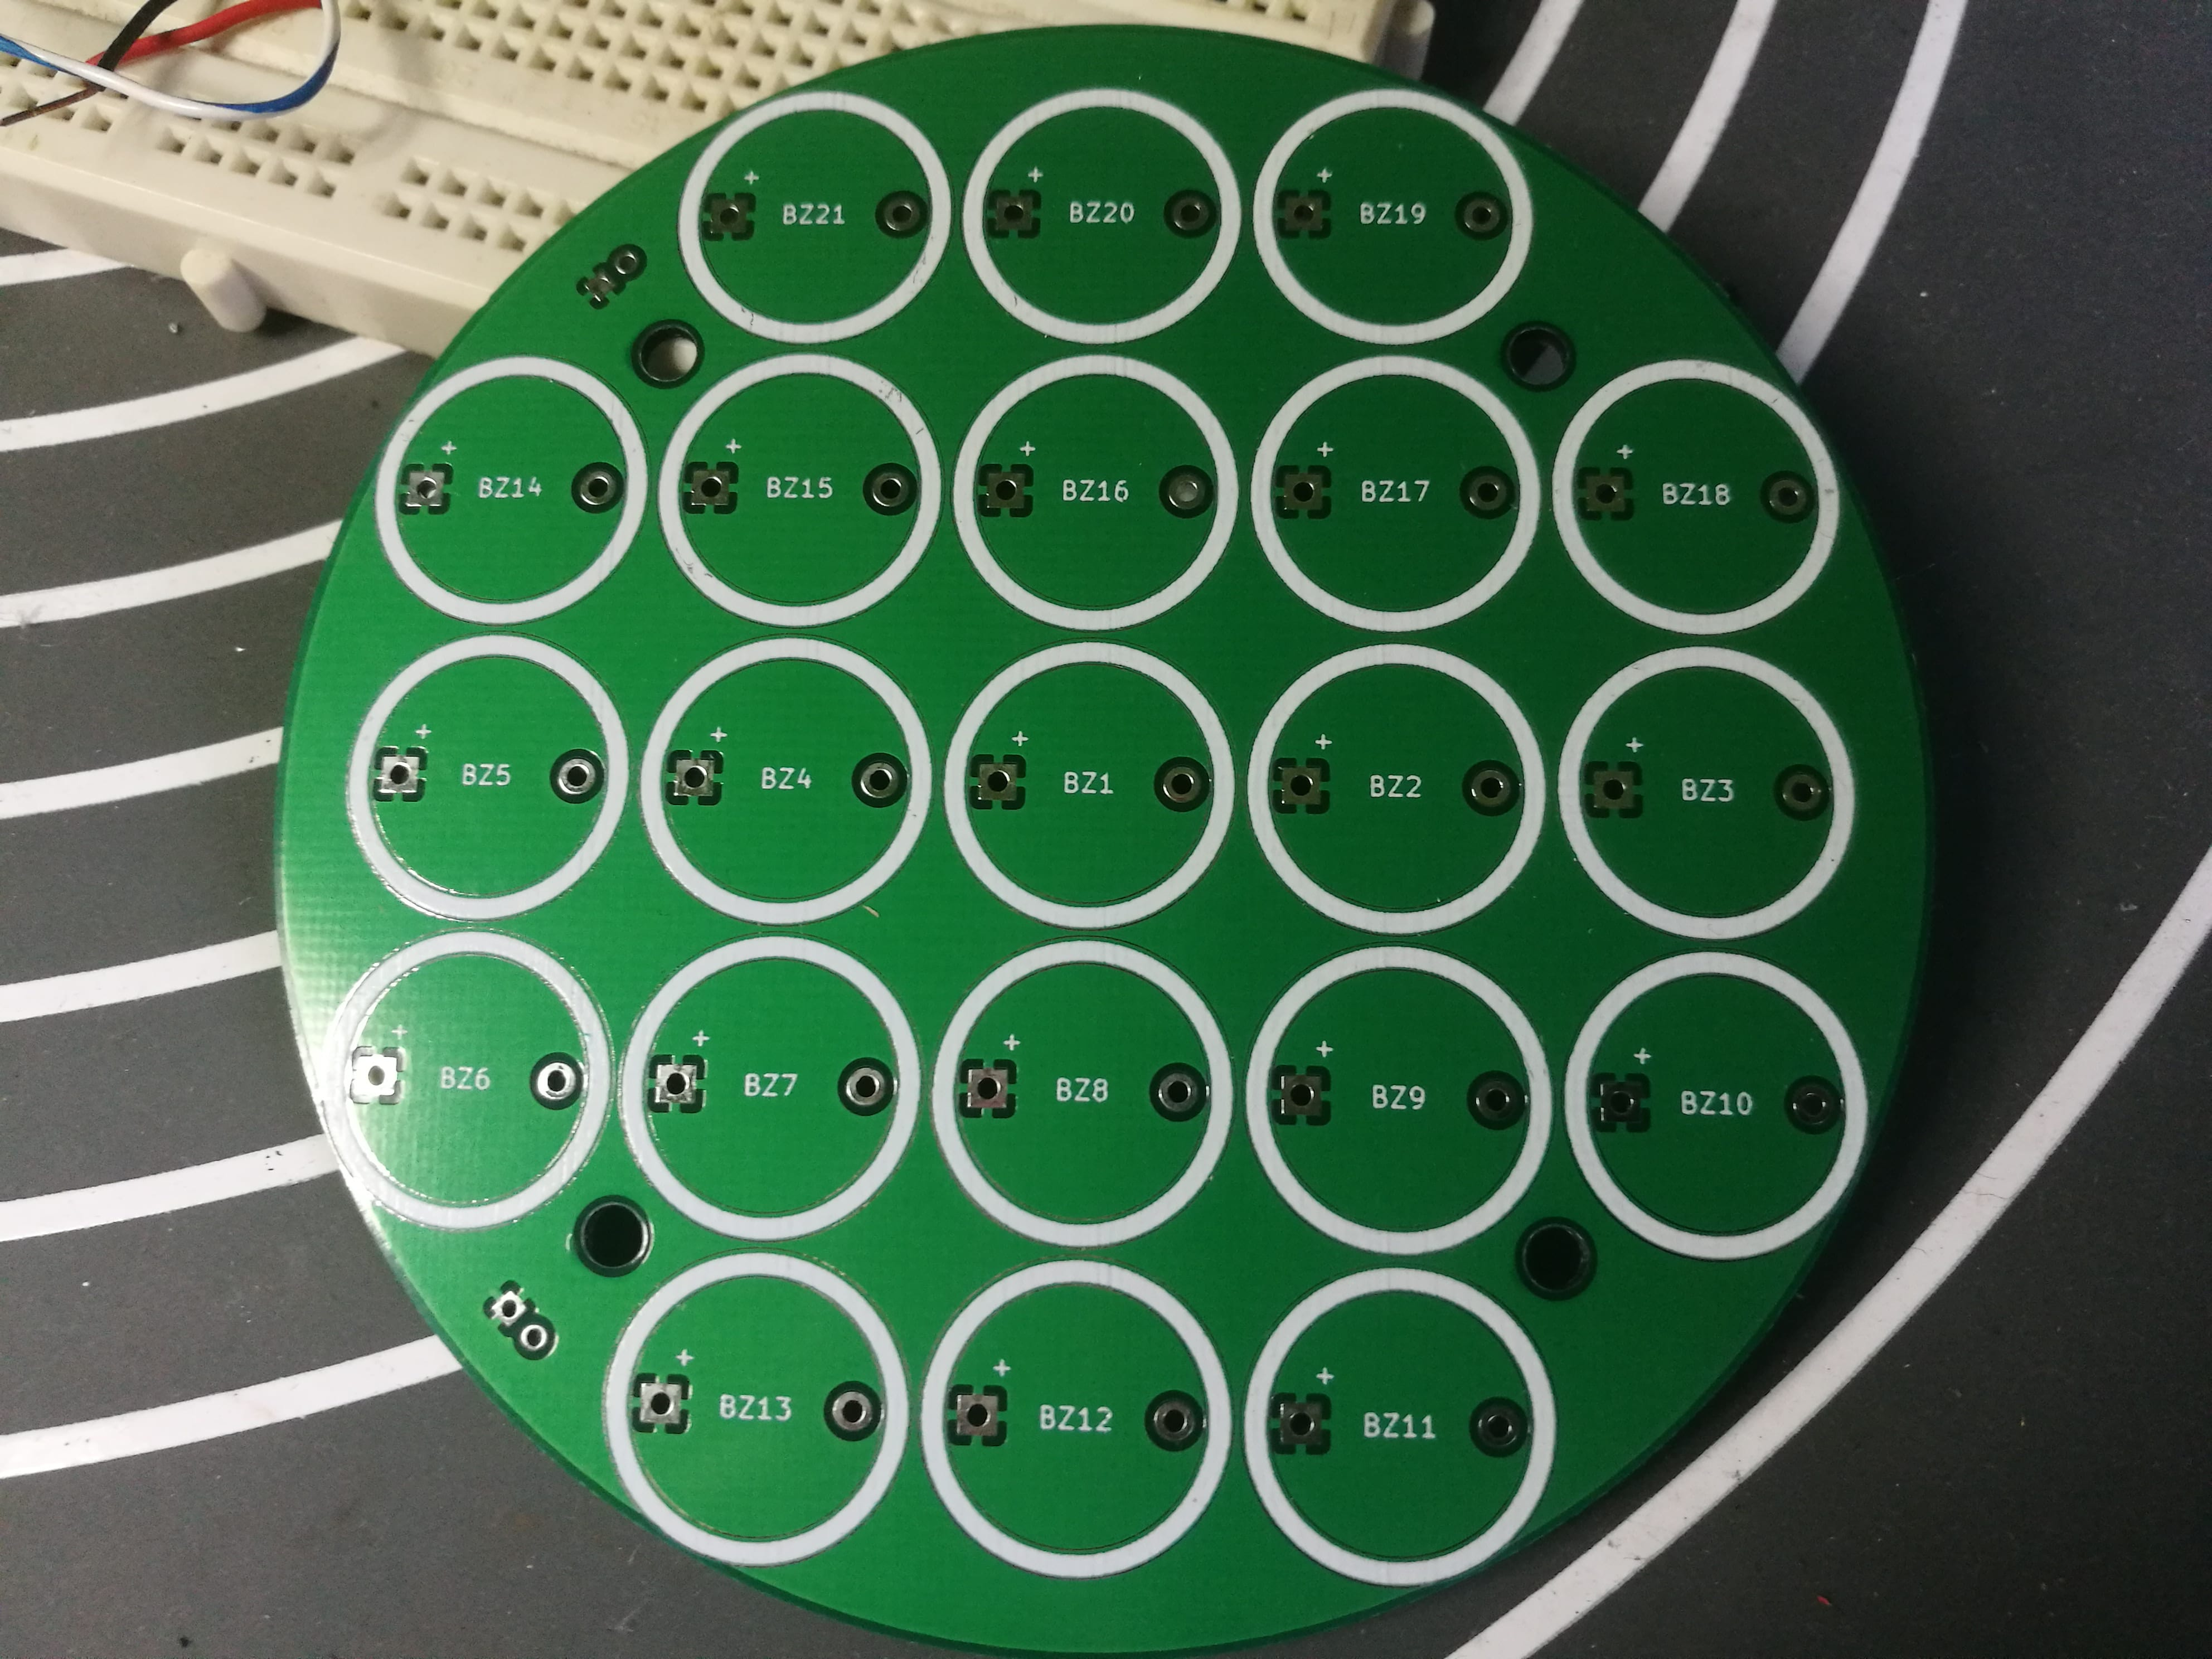
\includegraphics[width= \textwidth]{Figures/Implementation/TransducerArray/pcbfront.jpg}
    \caption{Front side of unpopulated PCB}
    \label{fig:pcbfrontunpop}
    \end{minipage}\hfill
    \begin{minipage}{0.49\textwidth}
    \centering
    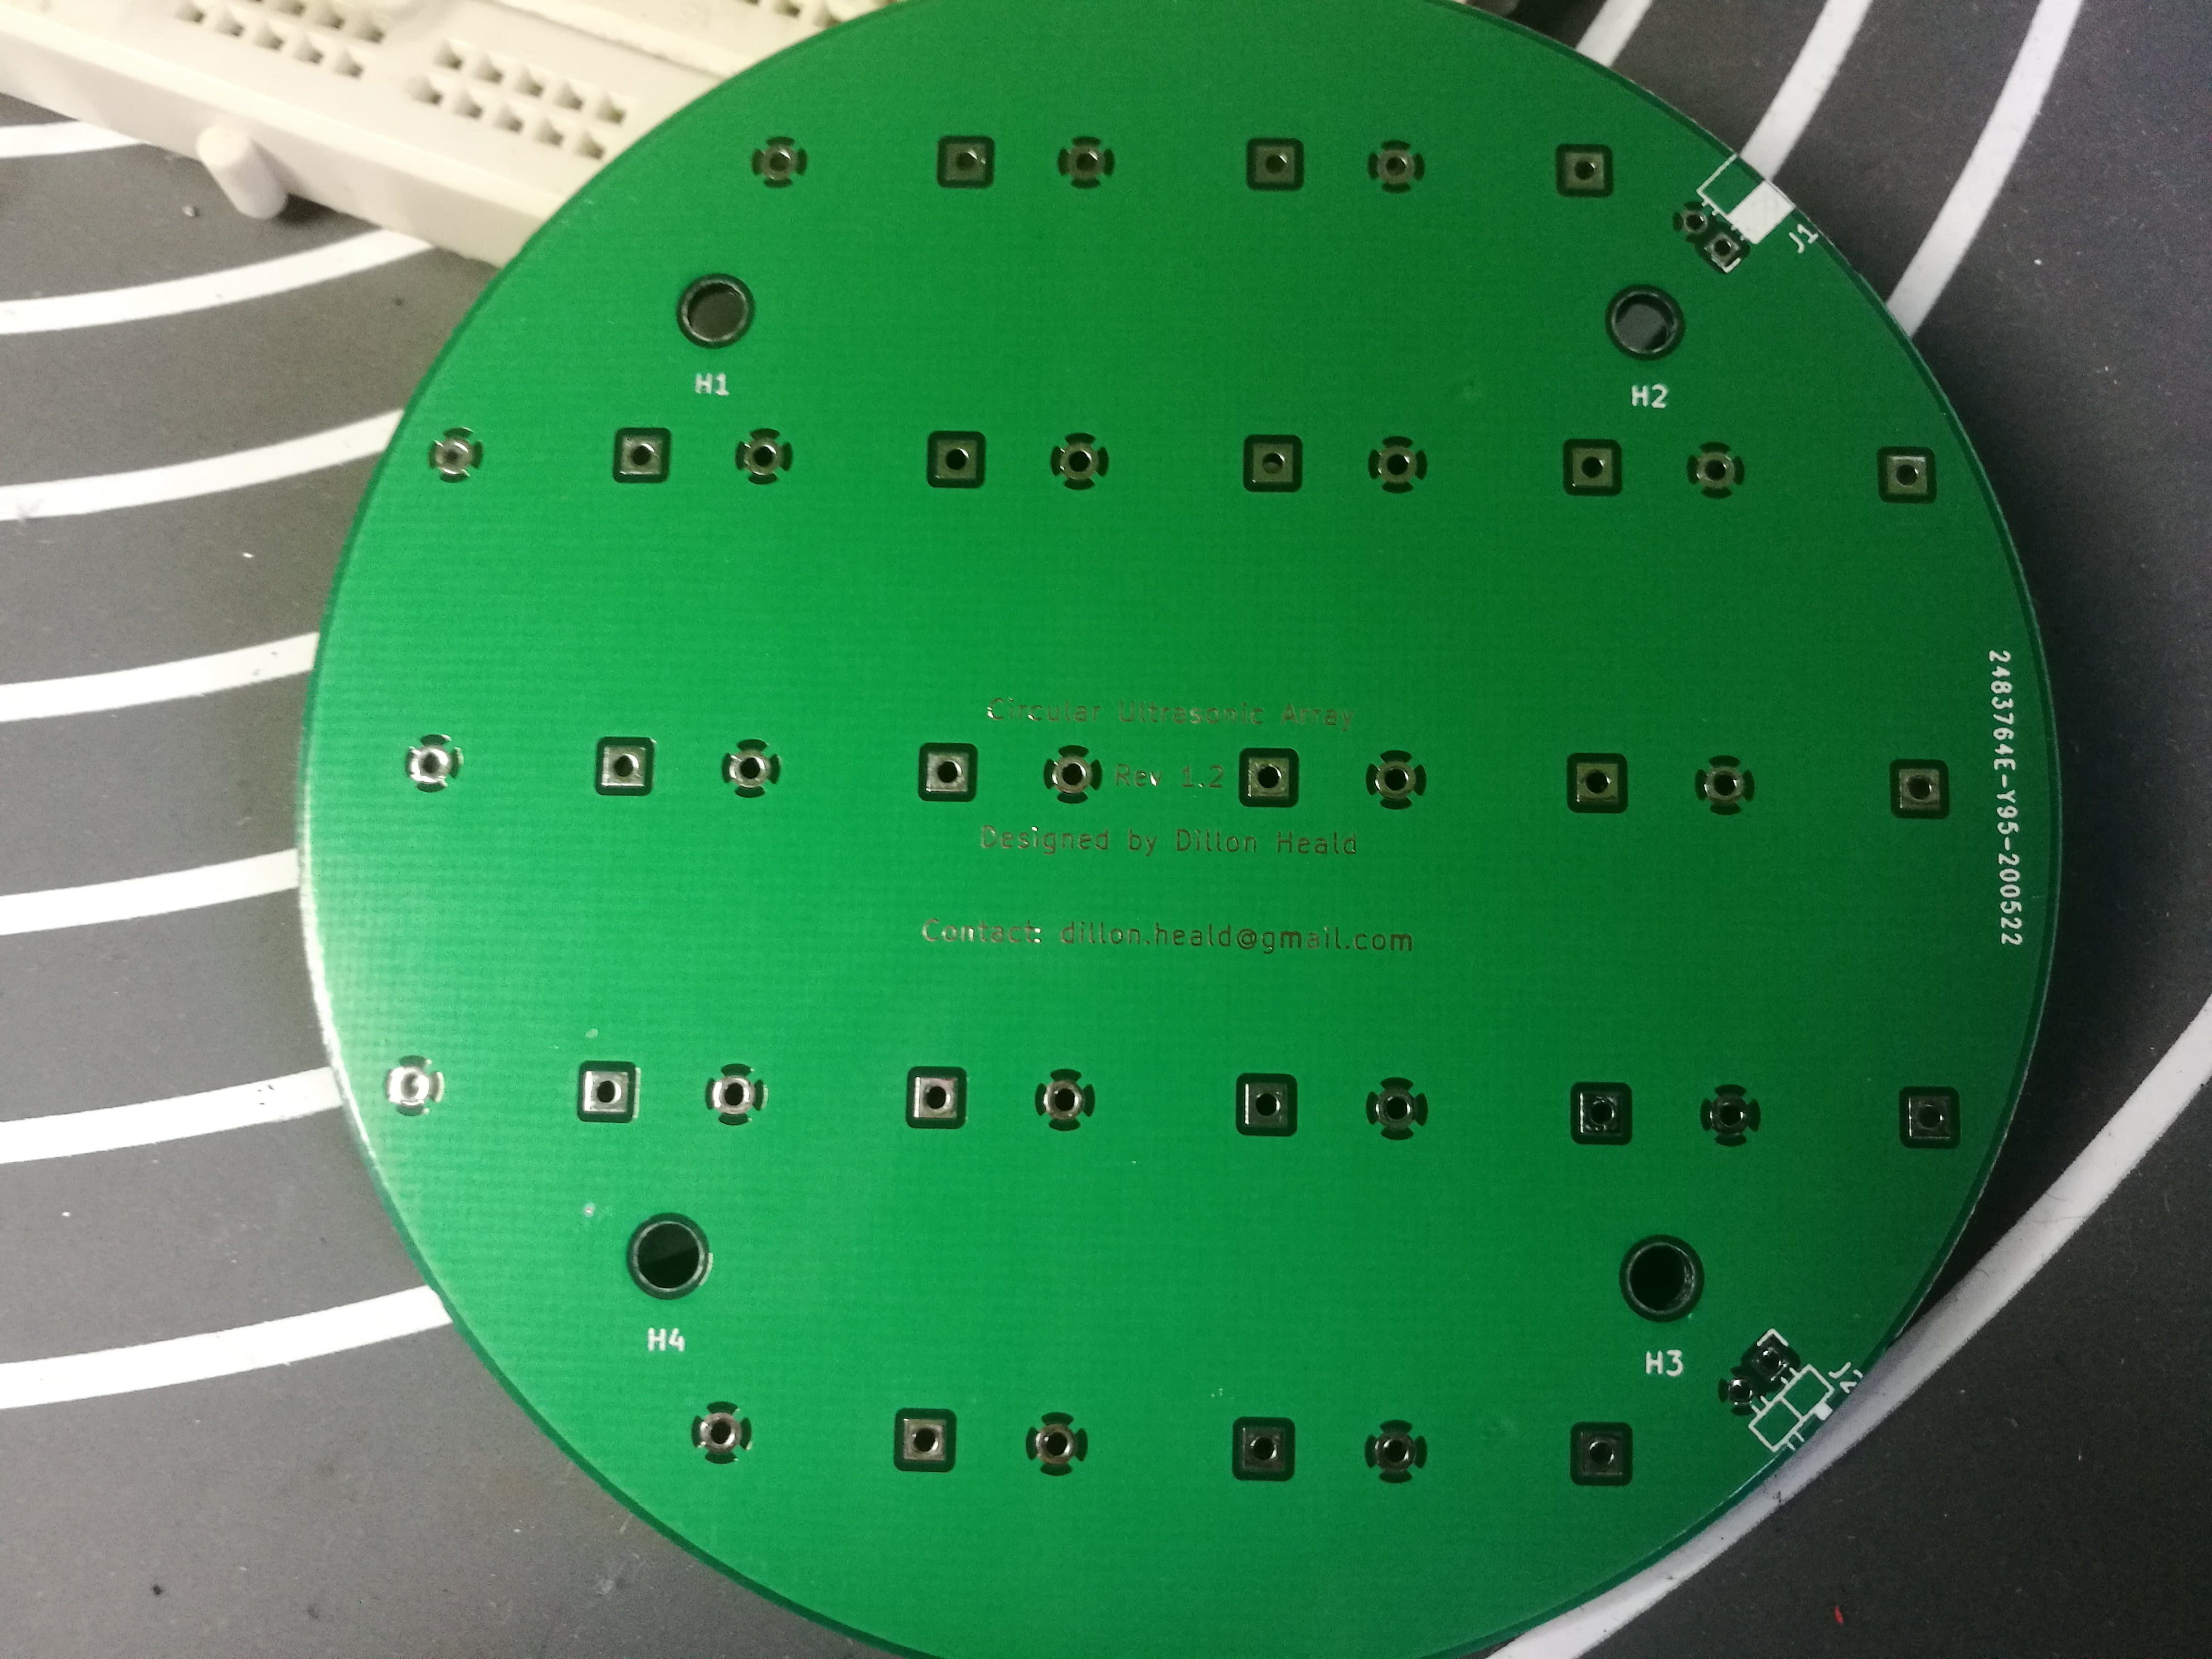
\includegraphics[width= \textwidth]{Figures/Implementation/TransducerArray/pcbback.jpg}
    \caption{Back side of unpopulated PCB}
    \label{fig:pcbbackunpop}
    \end{minipage}
    
\end{figure}


\begin{figure}[ht!]
\centering

    \begin{minipage}{0.49\textwidth}
    \centering
    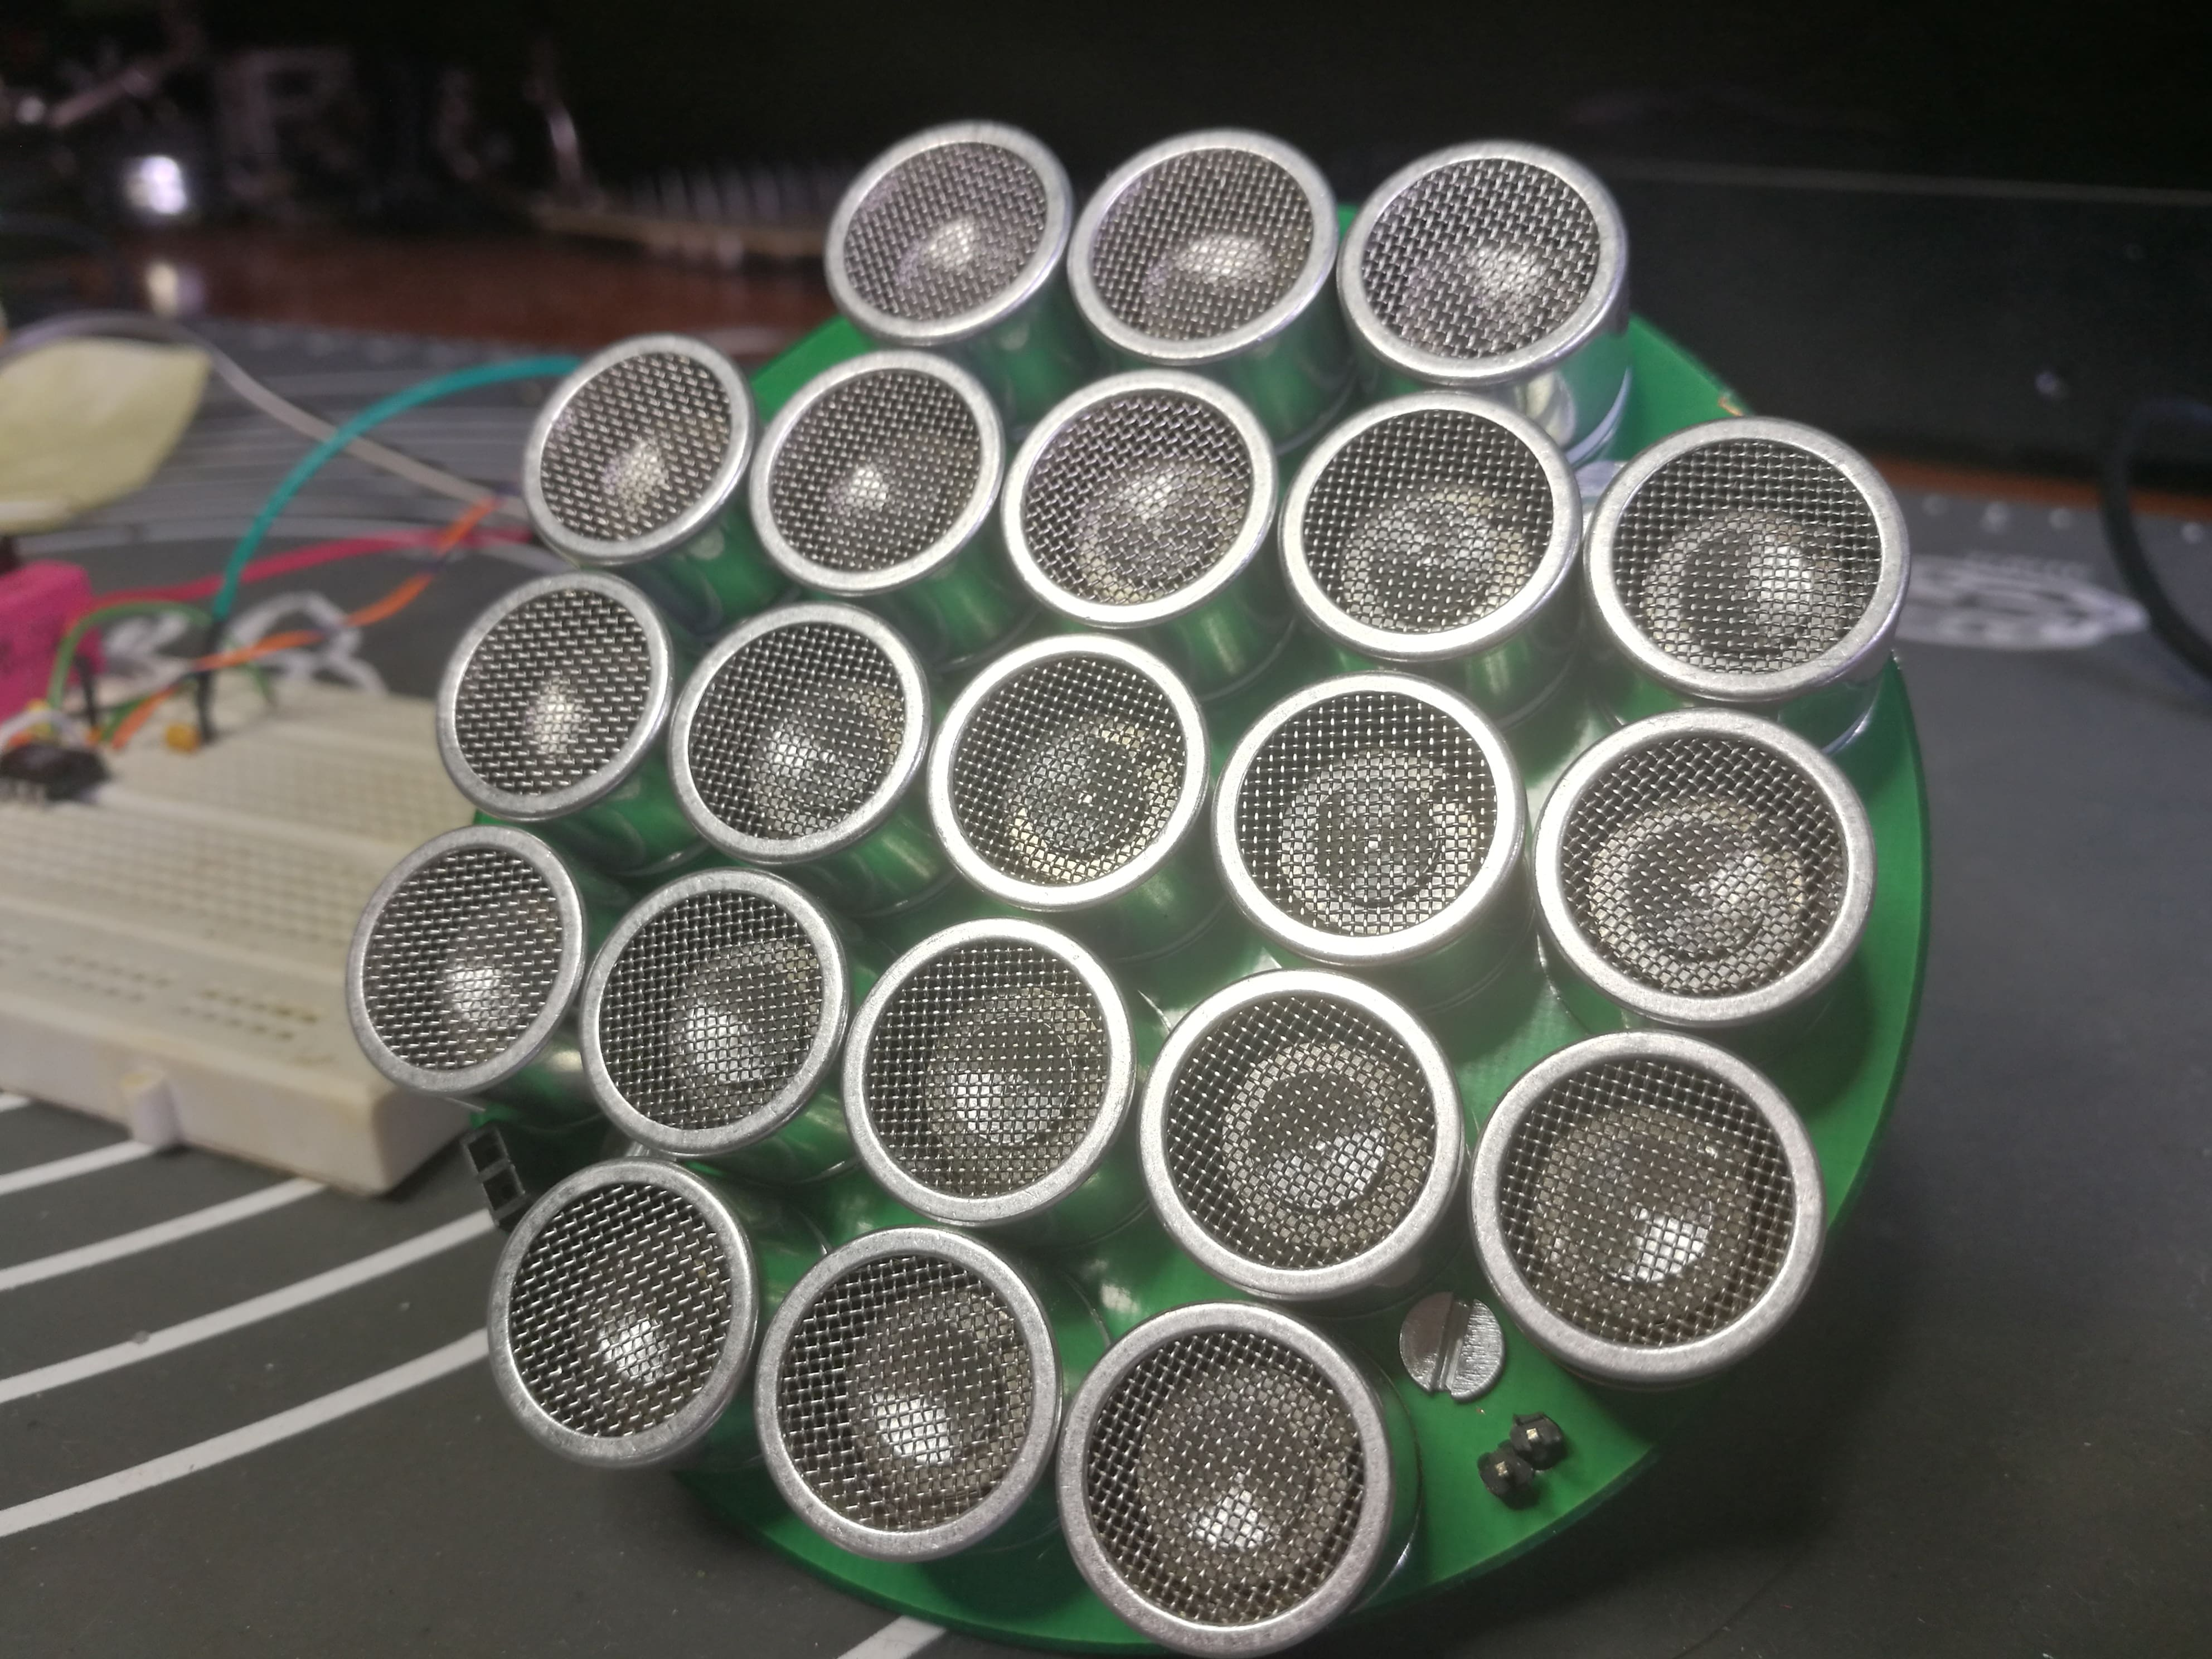
\includegraphics[width= \textwidth]{Figures/Implementation/TransducerArray/pcbdoneFrontdiag.jpg}
    \caption{Front side of populated PCB}
    \label{fig:pcbfront}
    \end{minipage}\hfill
    \begin{minipage}{0.49\textwidth}
    \centering
    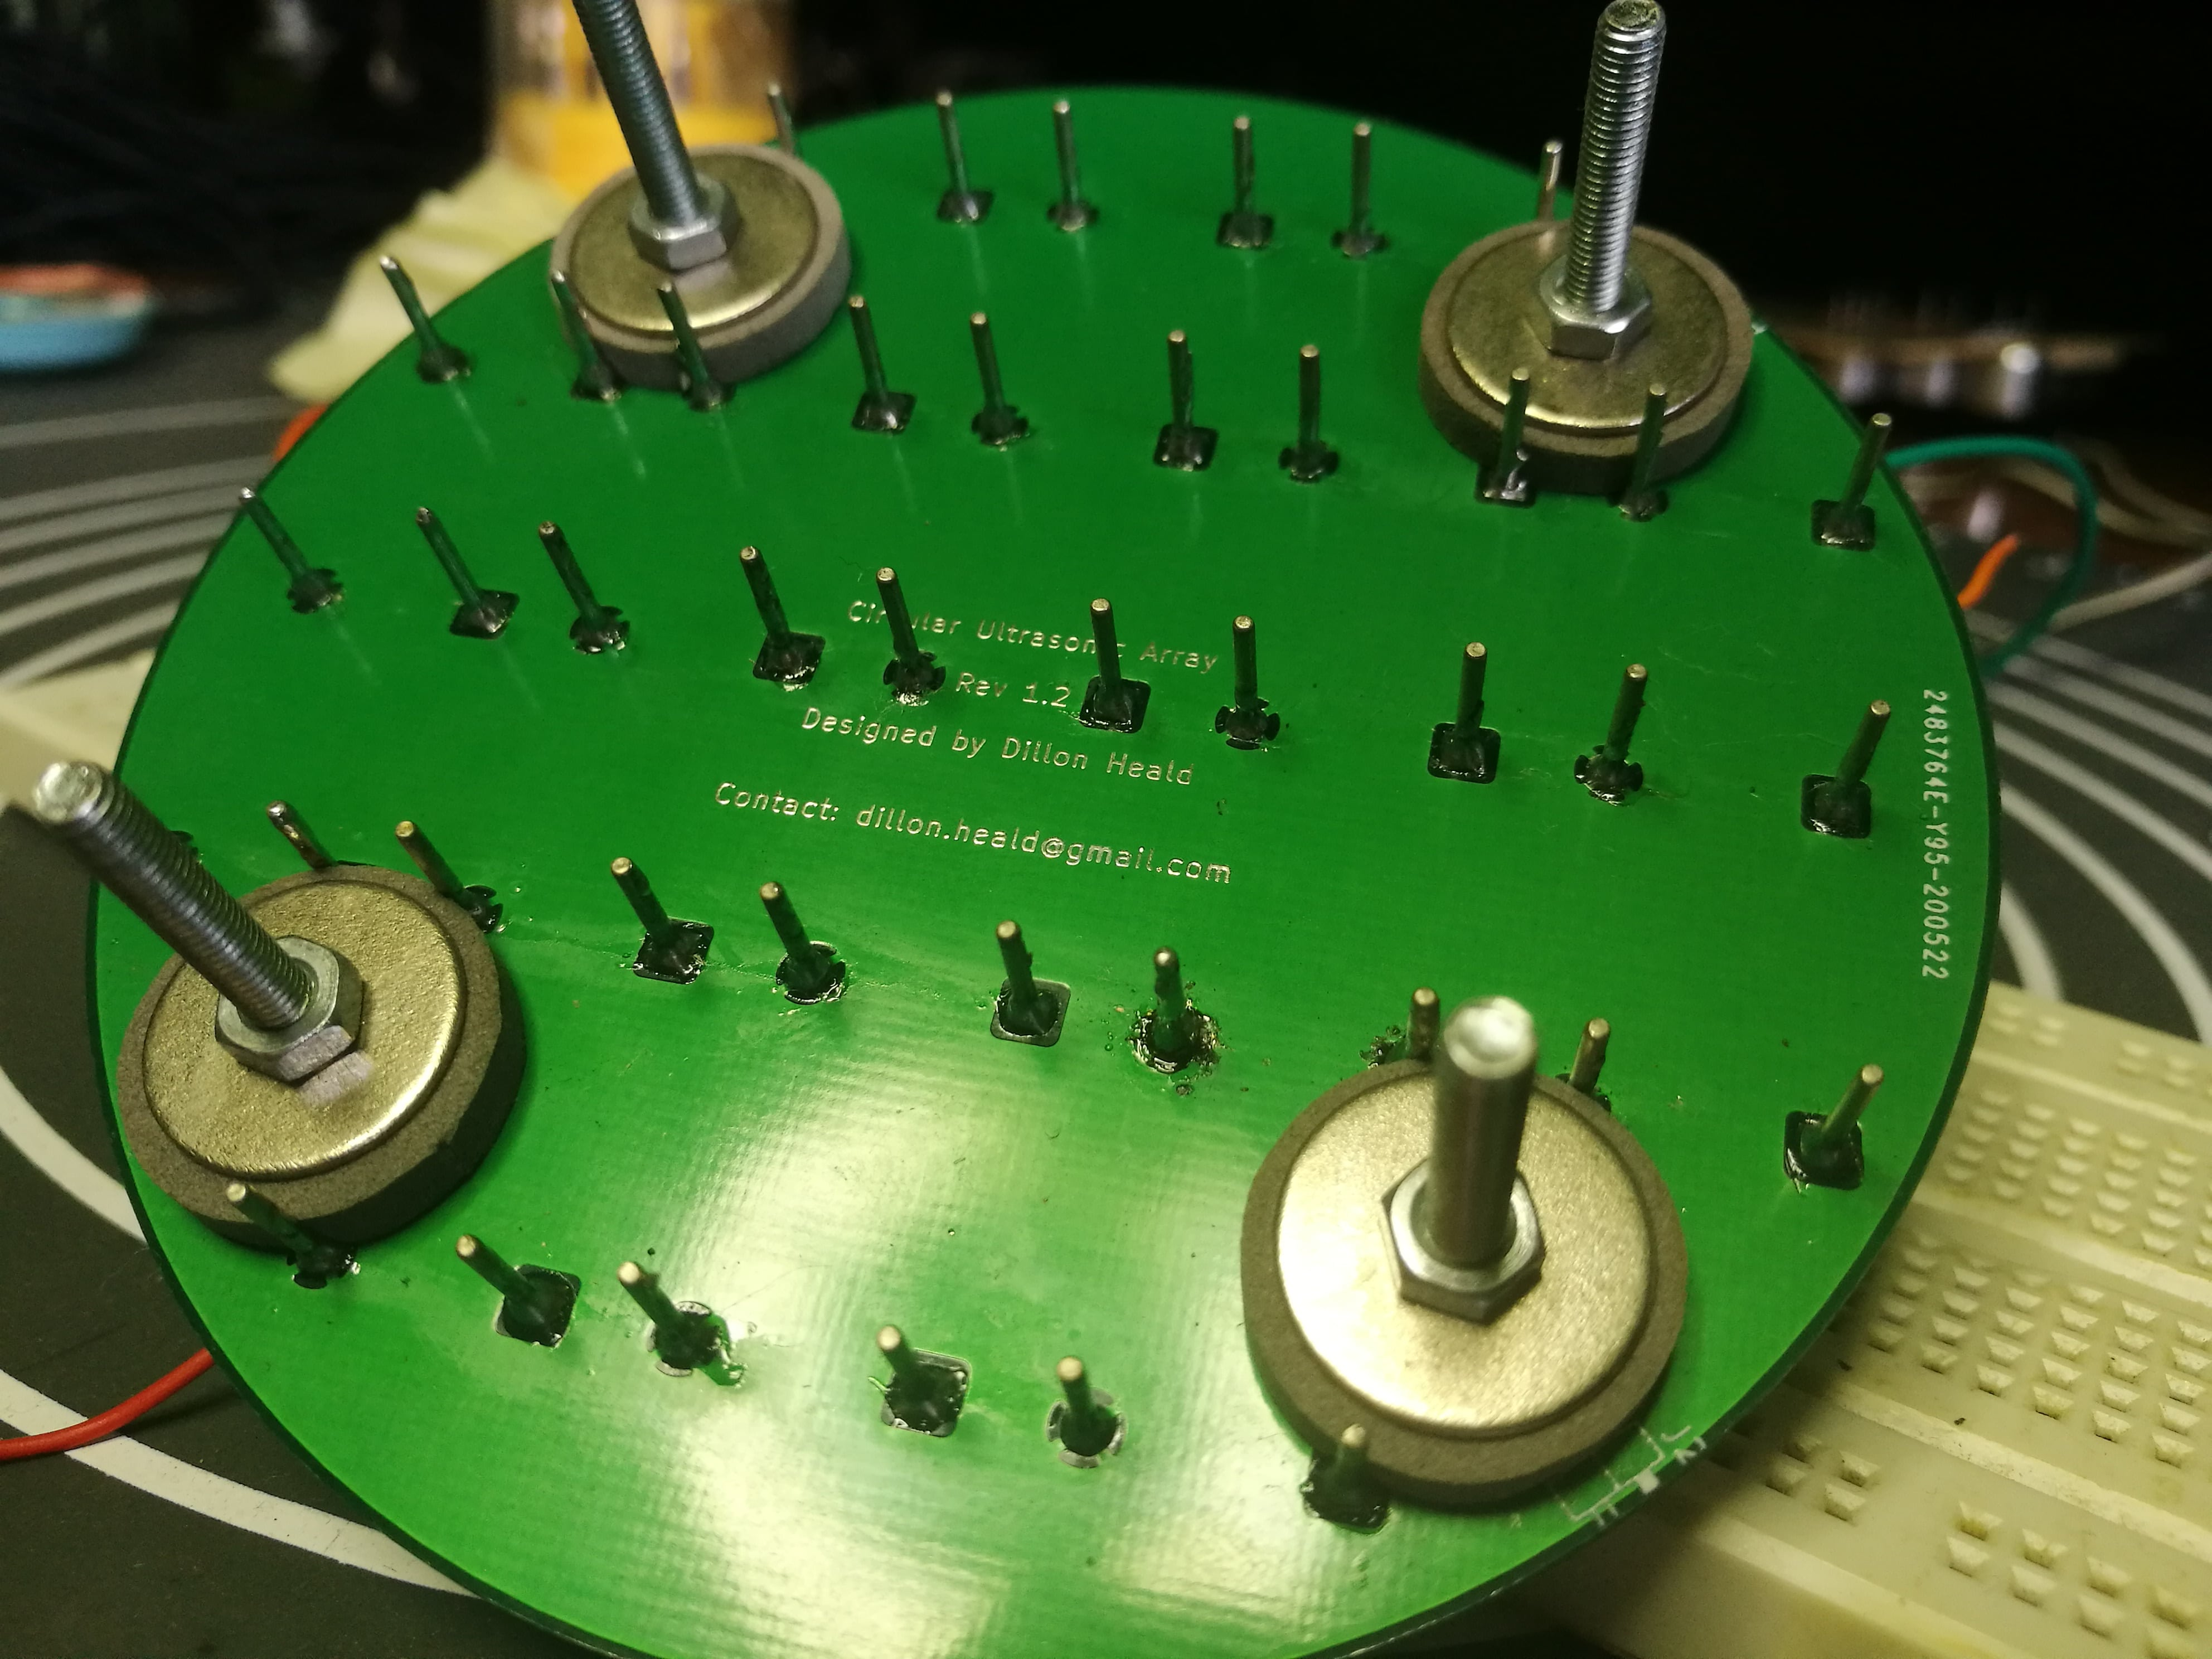
\includegraphics[width= \textwidth]{Figures/Implementation/TransducerArray/pcbdoneBackdiag.jpg}
    \caption{Back side of populated PCB}
    \label{fig:pcbback}
    \end{minipage}
    
\end{figure}

Once the PCB was populated, a 40 kHz tone was generated by the function generator and attached to the input of the PCB. Using 2 channels on a Tektronix 2246 oscilloscope, a receiver transducer was attached to one probe while the other probe was attached to the PCB's input signal allowing the output ultrasonic waves to be analysed and tested for any faults. The receiver transducer was passed over each emitting transducer and compared to the input signal, this test resulted in two transducers (BZ7 and BZ17 on the PCB) producing a $180^\circ$ phase shifted output as shown in figure \ref{fig:outphaseTran} where the top trace is the received signal and the bottom trace is the input signal.

\begin{figure}[ht!]
\centering

    \begin{minipage}{0.49\textwidth}
    \centering
    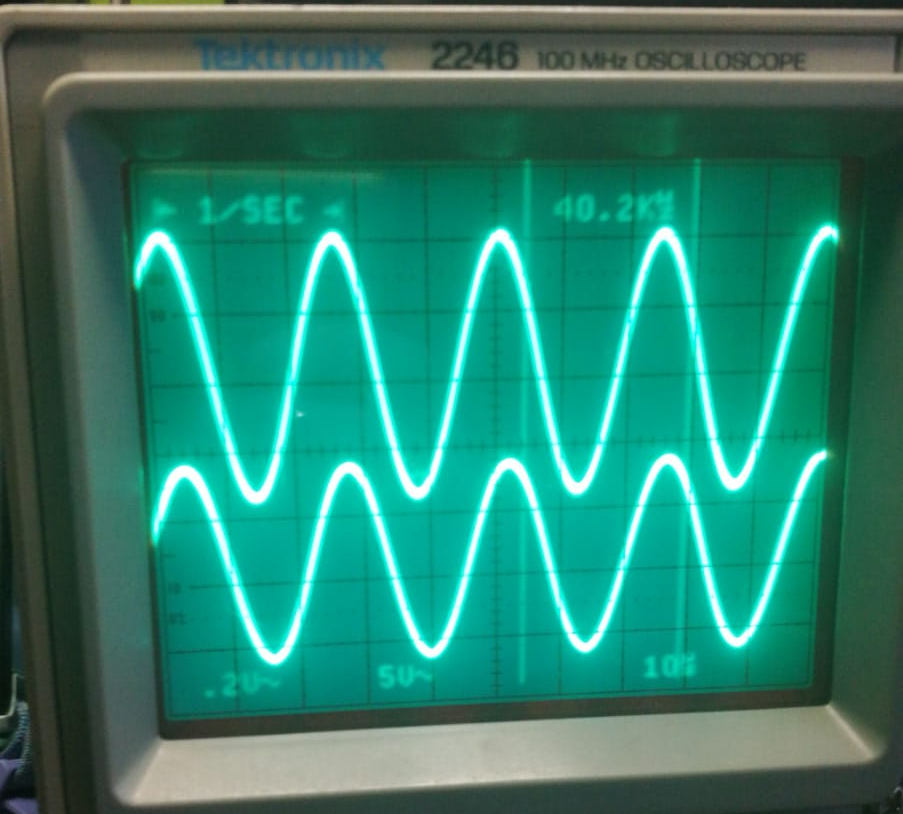
\includegraphics[width= \textwidth]{Figures/Implementation/TransducerArray/correctPhase.png}
    \caption{Transducer emitting in-phase output}
    \label{fig:inphaseTran}
    \end{minipage}\hfill
    \begin{minipage}{0.49\textwidth}
    \centering
    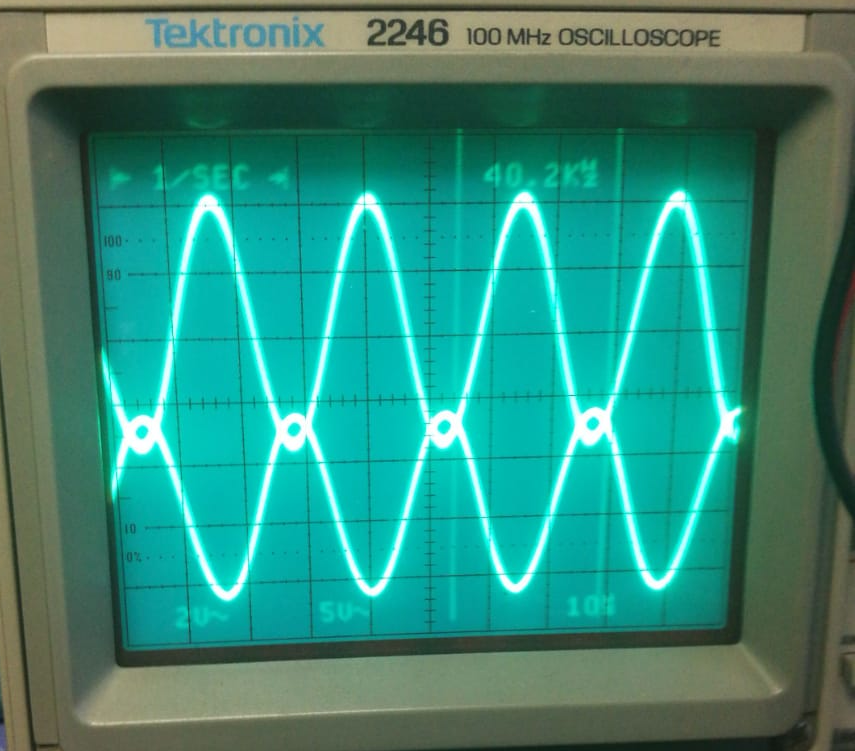
\includegraphics[width= \textwidth]{Figures/Implementation/TransducerArray/phaseInversion.png}
    \caption{Transducer emitting out of phase output}
    \label{fig:outphaseTran}
    \end{minipage}
    
\end{figure}

To correct this phase inversion, ultrasonic transducers 7 and 14 were removed from the PCB and replaced with known working transducers. Each element in the array was once again tested and all transducers emitted an in phase output.
\newpage
\subsection{Pre-processing development}
During signal simulation, julia code was used to create and process the signals involved in the directional audio system. Naturally, it would be ideal if the output of this julia code could be written to an audio port. Through some research, a library known as PortAudio was discovered which claimed to have exactly this ability, however; it is designed for C, C++ and requires a wrapper to work with julia. The wrapper \cite{russell_2016} allows for sampled signals to be written to the audio interface as long as they are values between $\pm1$. Adapting the code shown in the simulation section to record audio, process and play the processed output through the computers audio interface required a few adaption such as high pass filtering and signal level shifts and is shown in full in the appendix under listing \ref{lst:juliarecProPly}.
The result of this implementation produced a reduced in magnitude output due to the repeated integration which was corrected for by increasing the output amplitude by a tuned factor. Upon input into the modulator, passing through the amplifier and into the ultrasonic transducer array, the signal was heavily distorted. To troubleshoot this, the integration of the signal was removed and the signal was instead only shifted above zero and square-rooted. This resulted in a far less distorted output by the transducer array.
Since the output was now more intelligible, a new julia program was developed that only performed the signal shift and square-root operation on a generated tone of 2.5 kHz. This pre-processed tone could be adjusted in length up to 60 seconds as PortAudio has a limitation on the size of its output buffer. This code is used to generate the pre-processed audio for use in the beam sweep tests further elaborated on in the testing methodology section.
Figures \ref{fig:preprocessTdom} and \ref{fig:preprocessFdom} demonstrate the inputs and outputs of the pre-processing julia program using only square-root, filtering and level shifting processing.

\begin{figure}[ht!]
\centering

    \begin{minipage}{0.49\textwidth}
    \centering
    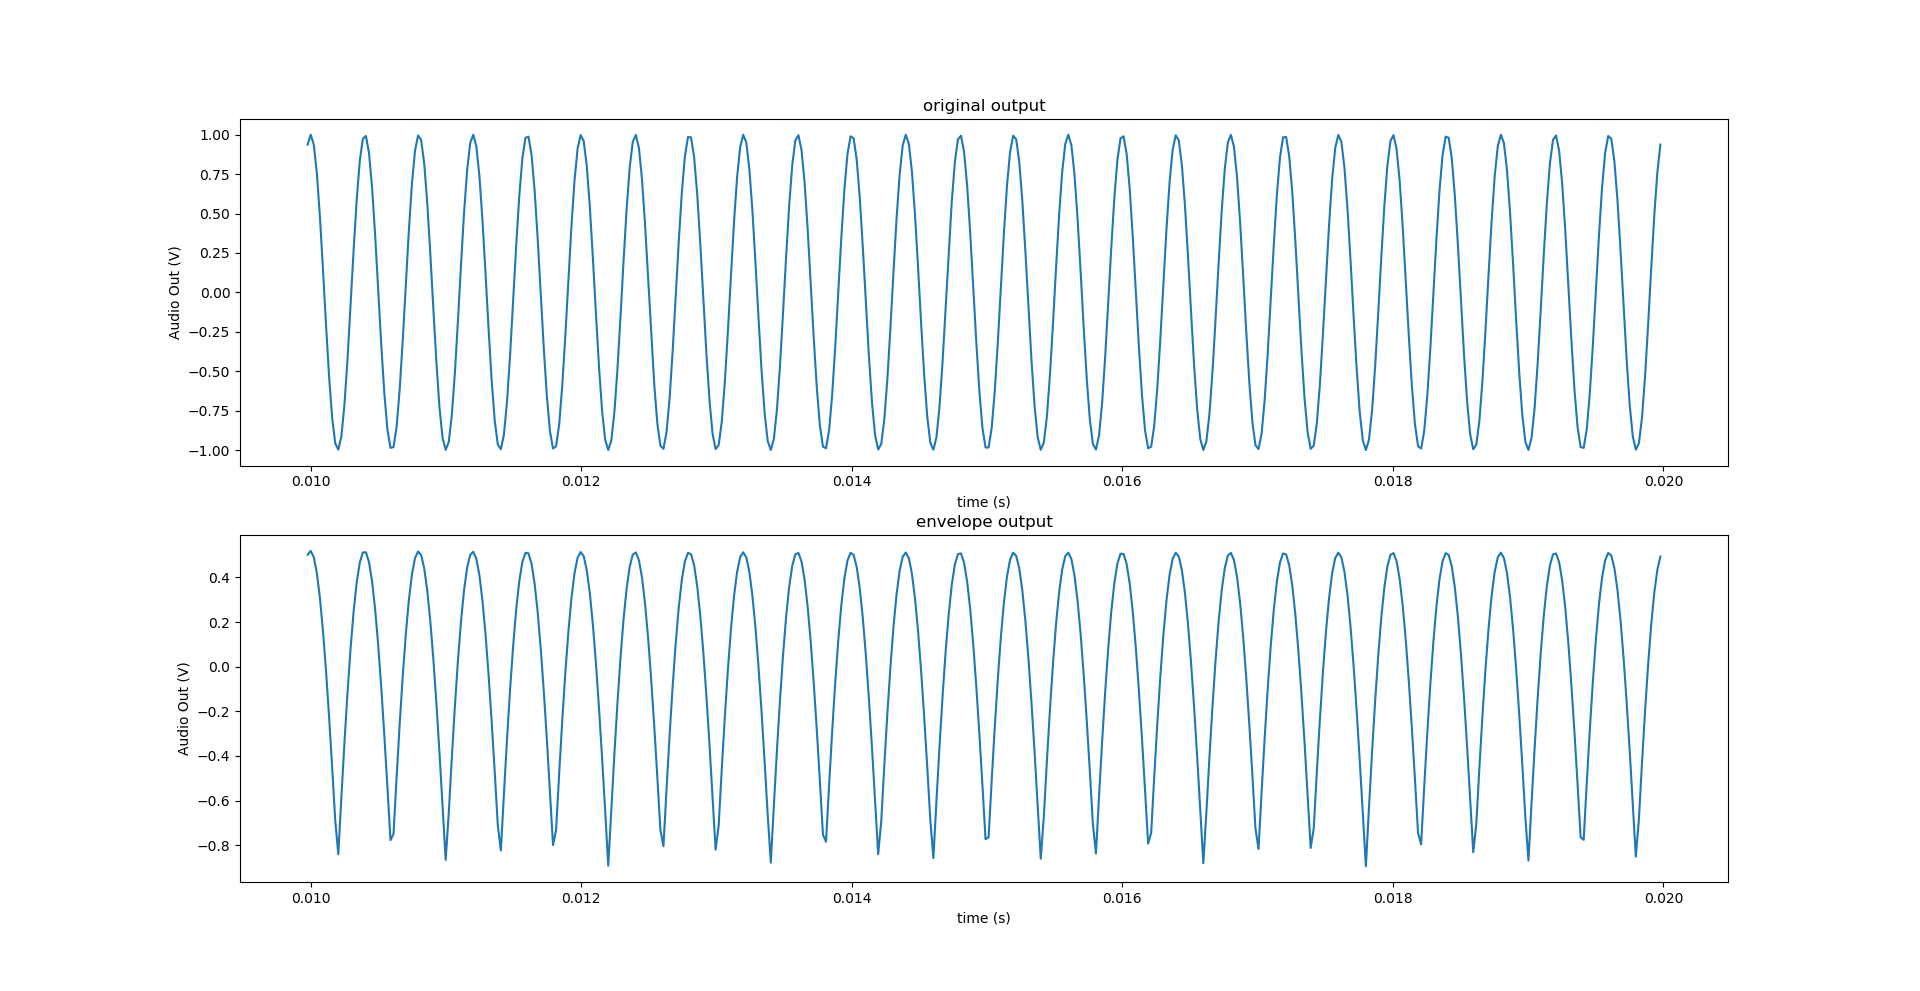
\includegraphics[width= \textwidth]{Figures/Implementation/Preprocessing/tdomainPreprocessing.png}
    \caption{Time domain representation of original tone and output pre-processed tone}
    \label{fig:preprocessTdom}
    \end{minipage}\hfill
    \begin{minipage}{0.49\textwidth}
    \centering
    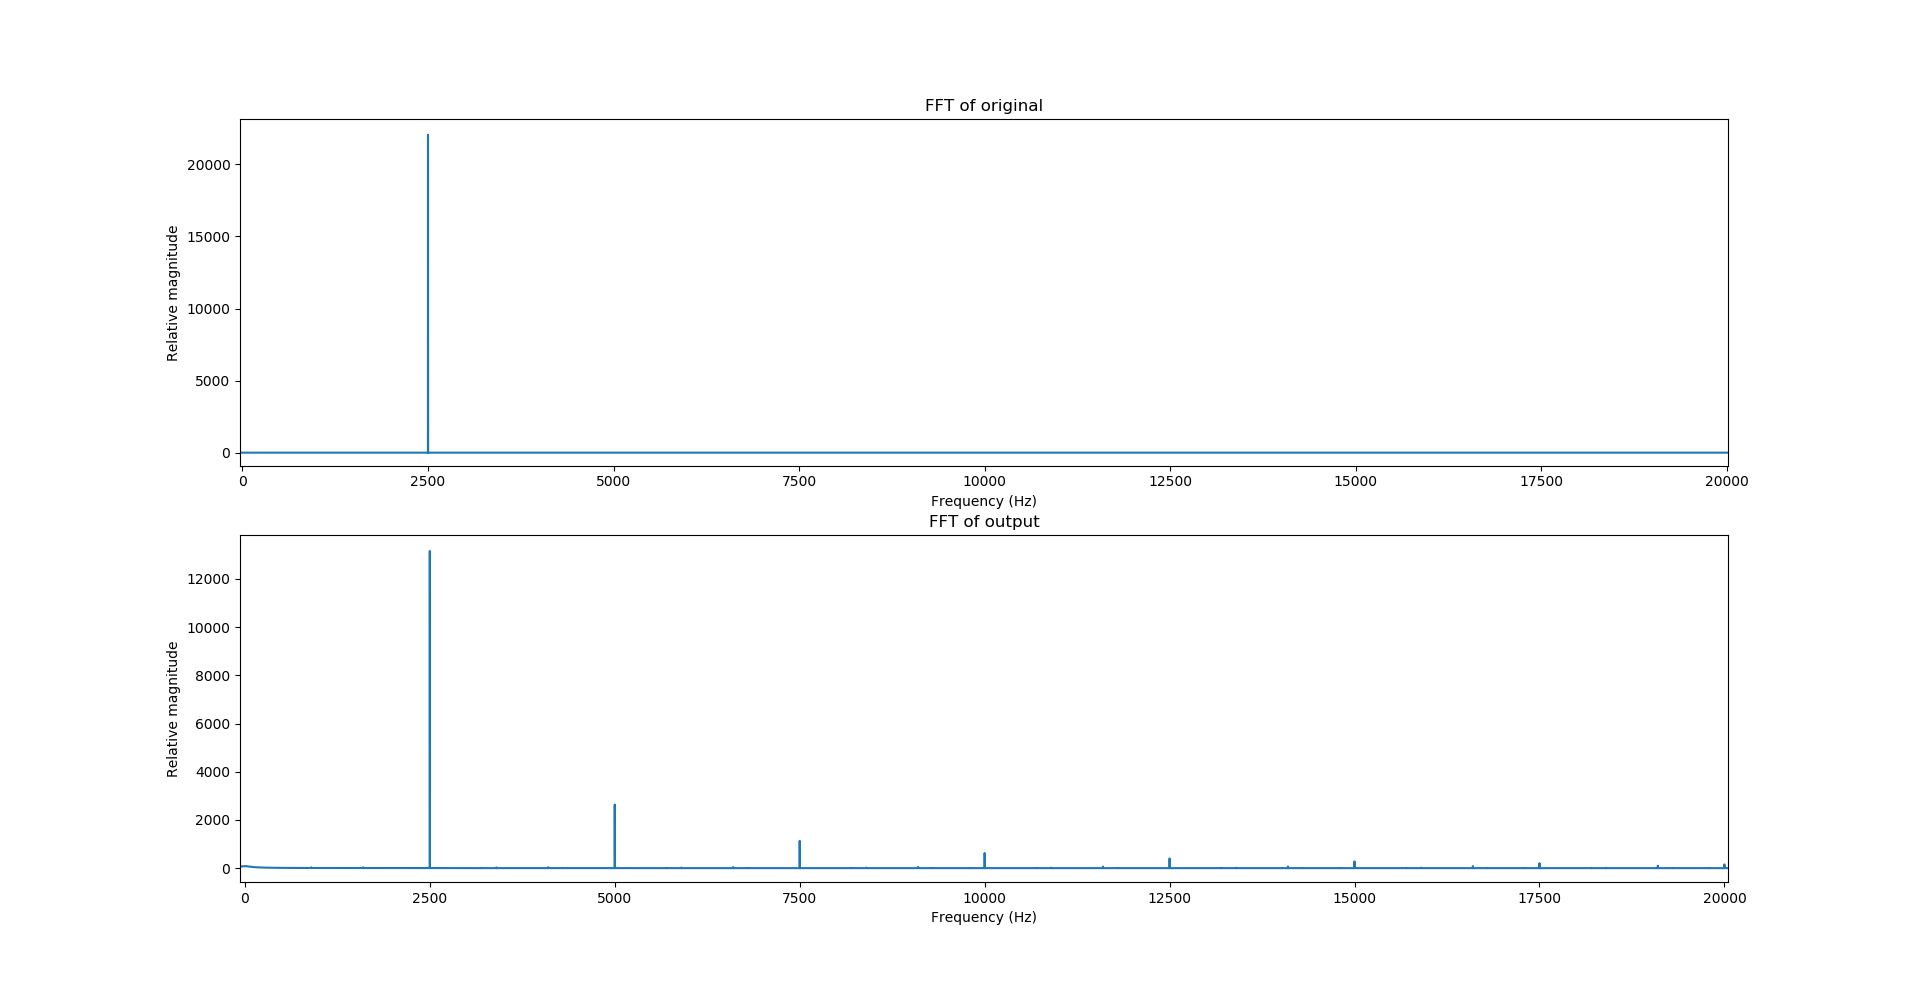
\includegraphics[width= \textwidth]{Figures/Implementation/Preprocessing/FFToutputPreprocessingPos.png}
    \caption{Frequency domain representation of original tone and output pre-processed tone}
    \label{fig:preprocessFdom}
    \end{minipage}
    
\end{figure}

%\begin{lstlisting}[caption={Conversion to time domain and double time derivative}\label{lst:doubledt},language=julia, style=jlcodestyle]

%\end{lstlisting}
